\documentclass{article}

\usepackage{amsmath}
\usepackage{amssymb}
\usepackage{physics}
\usepackage{graphicx}
\usepackage[perpage]{footmisc}

\setlength\parindent{0pt}

% \newcommand{\norm}[1]{\left\lVert#1\right\rVert}
\newcommand*\mean[1]{\bar{#1}}
% independent
\newcommand{\indep}{\rotatebox[origin=c]{90}{$\models$}}

\renewcommand{\thefootnote}{\fnsymbol{footnote}}

\DeclareMathOperator*{\argmax}{arg\,max}
\DeclareMathOperator*{\argmin}{arg\,min}
\DeclareMathOperator*{\mmax}{max}
\DeclareMathOperator*{\minf}{inf}
\DeclareMathOperator*{\msup}{sup}

\begin{document}

\title{Definitions and notations}
\author{Zhehao Wang}

\maketitle{}

\section{Calculus and linear algebra}

\subsection{Limit}

Let $f(x)$ be a function defined on an interval that contains $x = a$, except possibly at $x = a$, then we say that
$$
\lim\limits_{x \to a}{f(x) = L}
$$
if for every $\epsilon > 0$ there is some number $\delta > 0$ such that
$$
|f(x) - L| < \epsilon ~ \text{whenever} ~ 0 < |x - a| < \delta
$$

\subsection{Gradient}
Given $f(\vec{x})$ where $\vec{x} = (x_1, \dots, x_n)$ on $\mathbf{R}^n$
$$
\bigtriangledown f(a_1, \dots, a_n) = (\frac{\partial f}{\partial x_1}(a_1, \dots, a_n), \dots, \frac{\partial f}{\partial x_n}(a_1, \dots, a_n))
$$

\textbf{Intuition}: gradient is a vector (the rate of change of your function, when you move in a certain direction), which in a two-dimensional space, tangents the curve at a given point.

\subsection{Directional derivative}

$$
\bigtriangledown_v f(\vec{x}) = \lim\limits_{h \to 0}{\frac{f(\vec{x} + h\vec{v}) - f(\vec{x})}{h}}
$$

\textbf{Intuition}: the rate-of-change of a function $f(\vec{x})$ on direction $\vec{v}$.
Remember that this is a scalar (since we are given the direction).

$$
f'(x; u) = \bigtriangledown f(x)^{T} u
$$

Meaning gradient on a certain direction vector $u$ is $f(x)$'s directional derivative on $u$.

\subsection{Taylor expansion}

Every infinite differentiable function can be approximated by a series of polynomials.

Let $f(x)$ be a real function which is continuous on the closed interval $[a \dots b]$ and $n + 1$ times differentiable on the open interval $(a \dots b)$, let $\xi \in (a \dots b)$.

Then given any $x \in (a \dots b)$, there exists some $\eta \in \mathbb{R} : x \leq \eta \leq \xi$ or $\xi \leq \eta \leq x$ such that:

$$
f(x) = \sum_{k = 0}^{n} \frac{1}{k!} (x - \xi)^k f^{(k)}(\xi) + R_n
$$

Where $R_n = \frac{1}{(n + 1)!} (x - \xi)^{n + 1} f^{(n + 1)}(\eta)$ is the error term.

The expression

$$
f(x) = \sum_{n = 0}^{\infty} \frac{1}{n!} (x - \xi)^n f^{(n)}(\xi)
$$

where $n$ is taken to the limit is known as the Taylor series expansion of $f$ about $\xi$.

\subsection{Vector norm}
A norm is a function that assigns a stricly positive length or size to each vector in a vector space (except the zero vector which is assigned a length of 0).

\textbf{Absolute value norm} is a norm on the one-dimensional vector spaces formed by real or complex numbers.
$$
\norm{x} = |x|
$$

\textbf{Euclidean norm} on a Euclidean space $\mathbf{R}^n$ is such
$$
\norm{\vec{x}}_2 = \sqrt{x_1^2 + \dots + x_n^2}
$$

\textbf{Manhattan or taxicab norm}
$$
\norm{\vec{x}}_1 = \sum_{i = 1}^{n}{|x_i|}
$$

\textbf{$p$-norm}
$$
\norm{\vec{x}}_p = (\sum_{i = 1}^{n}{|x_i|^p})^{\frac{1}{p}}
$$
Note that when $p = 1$, we get Manhattan norm, and when $p = 2$, we get Euclidean norm.

When $p = \infty$
$$
\norm{\vec{x}}_{\infty} = {\mmax_{i}{|x_i|}}
$$

\subsection{argmax}

Points of the domain of some function at which the function values are maximized.

Given an arbitrary set $X$, a totally ordered set $Y$ and a function $f: X \to Y$, the $\argmax$ over some subset $S$ of $X$ is defined by
$$
\argmax_{x \in S \subseteq X}{f(x)} = \{x ~ | ~ x \in S \land \forall y \in S : f(y) \leq f(x)\}
$$

\subsection{Dot product, inner product}

Maps two equal-size vectors to a real value.

$$
\cdot : \mathbf{R}^d \times \mathbf{R}^d \to \mathbf{R}
$$

Defined geometrically, given two vectors $a$ and $b$,

$$
a \cdot b = \norm{a} \norm{b} cos(\theta)
$$

where $\theta$ is the angle between $a$ and $b$.

Defined algebraically,

$$
a \cdot b = a^{T}b
$$

\subsection{Inner product space / pre-Hilbert space, Hilbert space}

An \textbf{inner product space} (over reals) is a vector space $\mathbb{V}$ and an \textbf{inner product}, which is a mapping

$$
\langle . , . \rangle : \mathbb{V} \times \mathbb{V} \to \mathbf{R}
$$

This space has the properties that $\forall x, y, z \in \mathbb{V}$ and $a, b \in \mathbf{R}$,
\begin{itemize}
  \item symmetry: $\langle x, y \rangle = \langle y, x \rangle$
  \item linearity: $\langle a x + b y , z \rangle = a \langle x z \rangle + b \langle y , z \rangle$
  \item positive-definitiveness: $\langle x , x \rangle \geq 0$. And $\langle x , x \rangle = 0 \Longleftrightarrow x = 0$
\end{itemize}

A \textbf{norm} on the inner product space can then be defined as

$$
\norm{x} = \sqrt{\langle x , x \rangle}
$$

\textbf{Parallelogram law} states that a norm can be written in terms of an inner product on $\mathbb{V}$ iff $\forall x, x' \in \mathbb{V}$,

$$
2 \norm{x}^2 + 2 \norm{x'}^2 = \norm{x + x'}^2 + \norm{x - x'}^2
$$

And if it can be, the inner product is given by the \textbf{polarization identity}

$$
\langle x , x' \rangle = \frac{\norm{x}^2 + \norm{x'}^2 - \norm{x - x'}^2}{2}
$$
\\
\\
\textbf{Pythagorean theorem} states that two vectors are \textbf{orthogonal} if $\langle x , x' \rangle$ = 0, denoted as $x \perp x'$.
And $x$ is orthogonal to a set $S$ if for all $s \in S$, $x$ is orthogonal to $s$.

If $x \perp x'$, then $\norm{x + x'}^2 = \norm{x}^2 + \norm{x'}^2$
\\
\\
Roughly, \textbf{projection onto a plane} can then be defined as for $x \in \mathbb{V}$, let $M$ be a subspace of inner product space $\mathbb{V}$, then $m_0$ is the projection of $x$ onto $M$ if $m_0 \in M$ and is the closest point to $x$ in $M$.
Meaning $\forall m \in M$, $\norm{x - m_0} \leq \norm{x - m}$.

A Hilbert space is a complete\footnote{a space is complete if all Cauchy sequences in the space converge.} inner product space.
E.g. $\mathbf{R}^d$ and the standard inner product. Any finite dimensional inner product space is a Hilbert space.

The \textbf{projection theorem} suggests, for a Hilbert space $\mathbf{H}$ , $M$ is a closed subspace of $\mathbf{H}$, for any $x \in \mathbf{H}$, there exists a unique $m_0 \in M$ for which

$$
\norm{x - m_0} \leq \norm{x - m} ~ \forall m \in M
$$

This $m_0$ is called the orthogonal projection of $x$ onto $M$.
Furthermore, $m_0 \in M$ is the projection of $x$ onto $M$ iff $x - m_0 \perp M$.

Projection reduces norm: let $M$ be a closed subspace of $\mathbf{H}$.
For any $x \in \mathbf{H}$, let $m_0$ be the projection of $x$ onto $M$, then $\norm{m_0} \leq \norm{x}$ with equality only when $m_0 = x$. \footnote{think Pythagorean theorem on a $\mathbf{R}^2$ space}

\subsection{Cauchy-Schwarz inequality}

Given two vectors $u$ and $v$

$$
|\langle u , v \rangle|^2 \leq |\langle u , u \rangle| \cdot |\langle v , v \rangle|
$$

Where $|\langle u , u \rangle|$ is the inner product.
The equality holds only when $u$ and $v$ are linearly independent (parallel).



\subsection{Jacobian matrix}

\textbf{Jacobian matrix} is the matrix of all first-order partial derivatives of a vector-valued function.

Suppose $\vec{f} : \mathbf{R}^n \to \mathbf{R}^m$, the Jacobian matrix $\vec{J}$ of $\vec{f}$ is defined as follows

$$
\vec{J} = \begin{bmatrix} ~ \frac{\partial \vec{f}}{\partial x_1} ~ \dots ~ \frac{\partial \vec{f}}{\partial x_n} ~ \end{bmatrix}
$$

or component-wise $\vec{J}_{ij} = \frac{\partial \vec{f_i}}{\partial x_j}$, meaning

$$
\vec{J} = 
 \begin{bmatrix}
  \frac{\partial \vec{f_1}}{\partial x_1} ~ \dots ~ \frac{\partial \vec{f_1}}{\partial x_n} \\
  \dots \\
  \frac{\partial \vec{f_m}}{\partial x_1} ~ \dots ~ \frac{\partial \vec{f_m}}{\partial x_n}
 \end{bmatrix}
$$

\subsection{Order of a matrix}



\subsection{Inversibility of a matrix}



\subsection{Eigenvalue, eigenvector}

An \textbf{eigenvalue} of a \textbf{linear transformation} \footnote{Think square transformation matrix} is a non-zero vector that changes by only a scalar factor when that linear transformation is applied to it.

Meaning the set of $\vec{v}$ that satisfies

$$
T(\vec{v}) = \lambda \vec{v}
$$

Where $T$ is the linear transformation, $\lambda$ is a scalar and called \textbf{eigenvalue}.

We can compute the eigenvalues $\lambda$ of a square matrix $A$ of size $n$ by solving this \textbf{determinant}

$$
|A - \lambda I| = 0
$$

Where $I$ is the \textbf{identity matrix (unit matrix)} of size $n$.

For each eigenvalue $\lambda$, we can then solve its (corresponding set of) eigenvectors $\vec{v}$ using

$$
(A - \lambda I) \cdot \vec{v} = 0
$$

\textbf{Intuition}: applying a linear transformation on an eigenvector of that linear transformation yields a vector that is parallel to this eigenvector (multiplier: eigenvalue).

\subsection{Positive-definite}

A \textbf{symmetric} $n \times n$ real matrix is positive definite if the scalar $z^{T} M z$ is strictly positive for every non-zero column vector $z \in \mathbf{R}^n$.

The identity matrix $I$ is positive definite.

For any real invertible matrix $A$, the product $A^{T} A$ is a positive definite matrix.

\subsection{Convexity}

A \textbf{set} $C$ is \textbf{convex} if for any $x_1, x_2 \in C$ and any $\theta$ with $0 \leq \theta \leq 1$ we have

$$
\theta x_1 + (1 - \theta) x_2 \in C
$$

\textbf{Intuition}: for all $x_1$, $x_2$ in $C$, all the points on the line segment connecting points $x_1$, $x_2$ are in $C$.
\\
\\
A \textbf{function} $f: \mathbf{R}^n \to \mathbf{R}$ is \textbf{convex} if $\text{dom}$ $f$ is a convex set and if for all $x, y \in \text{dom} ~ f$, and $0 \leq \theta \leq 1$, we have

$$
f(\theta x + (1 - \theta) y) \leq \theta f(x) + (1 - \theta) f(y)
$$

\textbf{Intuition}: line segment connecting points $x$, $y$ on the graph of $f$ does not cross the graph of $f$.

Examples:
\begin{itemize}
  \item $f(x) = a x + b$ is both convex and concave on $\mathbf{R}$ for all $a, b \in \mathbf{R}$.
  \item $f(x) = |x|^p$ for $p \geq 1$ is convex on $\mathbf{R}$.
  \item $f(x) = e^{a x}$ for all $a$ is convex on $\mathbf{R}$.
  \item Every norm on $\mathbf{R}^n$ is convex.
  \item $f(x) = \text{max}\{ x \}$ is convex on $\mathbf{R}^n$.
\end{itemize}

A function $f$ is \textbf{strictly convex} if the line segment connecting any two points on the graph of $f$ lies strictly above the graph.

\begin{itemize}
  \item When a function is convex, if there is a local minimum, then it is a global minimum.
  \item When a function is strictly convex, if there is a local minimum, then it is the unique global minimum.
\end{itemize}

For a multivariate twice differentiable function, $h : \Theta \subset \mathbb{R}^d \to \mathbb{R}$, $d \geq 2$, the gradient vector is

$$
\bigtriangledown h(\theta) = 
\begin{pmatrix}
\frac{\partial h}{\partial \theta_1} (\theta) \\
\dots \\
\frac{\partial h}{\partial \theta_d} (\theta) \\
\end{pmatrix}
$$

A \textbf{Hessian matrix} of that function is

$$
\bigtriangledown^2 h(\theta) = 
\begin{pmatrix}
\frac{\partial^2 h}{\partial \theta_1 \partial \theta_1} (\theta) \dots \frac{\partial^2 h}{\partial \theta_1 \partial \theta_d} (\theta) \\
\dots \\
\frac{\partial^2 h}{\partial \theta_d \partial \theta_1} (\theta) \dots \frac{\partial^2 h}{\partial \theta_d \partial \theta_d} (\theta) \\
\end{pmatrix}
$$

$h$ is concave $\implies x^T \bigtriangledown^2 h(\theta) x \leq 0 ~ \forall x \in \mathbb{R}^d, \theta \in \Theta$.

$h$ is strictly concave $\implies x^T \bigtriangledown^2 h(\theta) x < 0 ~ \forall x \in \mathbb{R}^d, \theta \in \Theta$.

\subsection{The general optimization problem}

\textbf{Standard form}: minimize $f_0(x)$ subject to $f_i(x) \leq 0, ~ i = 1, \dots m$, $h_i(x) = 0, ~ i = 1, \dots m$.\footnote{Assuming the intersections of domains of all $f_i$ and $h_i$ is not empty.}
Where $f_0$ is the objective function and $x \in \mathbf{R}^n$ are the optimization variables.

We can replace $h(x) = 0$ with $h(x) \leq 0$ and $-h(x) \leq 0$, so we don't need the equality constraints.

The set of points satisfying the constraints is called the \textbf{feasible set}.

A point in the feasible set is called a \textbf{feasible point}.

If $x$ is feasible and $f_i(x) = 0$, then we say inequality constraint $f_i(x) \leq 0$ is \textbf{active} at $x$.

The \textbf{optimal value} $p^*$ of the problem is defined as

$$
p^* = \minf{\{ f_0(x) | x \in \text{feasible set}\}}
$$

$x^*$ is an \textbf{optimal point} (a solution to the problem) if $x^*$ is feasible and $f(x^*) = p^*$.


\subsection{Lagrangian duality}

Given a general optimization problem:

\begin{align*}
\text{minimize}       & f_0(x) \\
\text{subject to} ~ ~ & f_i(x) \leq 0, i = 1, \dots m.
\end{align*}

The \textbf{Lagrangian} for it is defined as

$$
L(x, \lambda) = f_0(x) + \sum_{i = 1}^{m}{\lambda_i f_i(x)}
$$

Where $\lambda_i$s are called \textbf{Lagrangian multipliers} (\textbf{dual variables}).\footnote{Irrelevant with convexity.}

\textbf{Supremum} over Lagrangian gives back encoding of objective and constraints:

\begin{align*}
\msup_{\lambda \succeq 0}{L(x, \lambda)} &= \msup_{\lambda \succeq 0}{( f_0(x) + \sum_{i = 1}^{m}{\lambda_i f_i(x)} )} \\
                                         &= \begin{cases}
                                              f_0(x), ~ ~ \text{when} ~ f_i(x) \leq 0 ~ \forall i \\
                                              \infty, ~ ~ \text{otherwise}
                                            \end{cases}
\end{align*}

And equivalent of the \textbf{primal form} of the optimization problem:

$$
p^* = \minf_{x}{ \msup_{\lambda \succeq 0}{(f_0(x) + \sum_{i = 1}^{m}{\lambda_i f_i(x)}} )}
$$

We get the \textbf{Lagrangian dual problem} by swapping the $\minf$ and $\msup$.

$$
d^* = \msup_{\lambda \succeq 0}{ \minf_{x}{(f_0(x) + \sum_{i = 1}^{m}{\lambda_i f_i(x)}} )}
$$

\textbf{Weak duality} $p^* \geq d^*$ holds for any optimization problem.
\footnote{Hint, for any general $f: W \times Z \to R$, this can be proved given $\minf_{w \in W}{f(w, z_0)} \leq f(w_0, z_0) \leq \msup_{z \in Z}{f(w_0, z)}$, add another $\msup$ to the leftmost term and $\minf$ to the rightmost term.}

\textbf{Duality gap} is $p^* - d^*$, for convex problems, we often have \textbf{strong duality}: $p^* = d^*$.

The \textbf{Lagrangian dual function} is

$$
g(\lambda) = \minf_{x}{L(x, \lambda)} = \minf_{x}{( f_0(x) + \sum_{i = 1}^{m}{\lambda_i f_i(x)} )}
$$

The dual function is always concave.\footnote{Pointwise min of affine functions}

Lagrangian dual function gives a lower bound on optimal solution:

\begin{align*}
p^* &\geq d^* = \msup_{\lambda \geq 0}{g(\lambda)} \\
p^* &\geq g(\lambda) ~ ~ \forall \lambda \geq 0
\end{align*}

The \textbf{Lagrangian dual problem} is a search for best lower bound on $p^*$: maximize $g(\lambda)$ subject to $\lambda \succeq 0$.

$\lambda$ is \textbf{dual feasible} if $\lambda \succeq 0$ and $g(\lambda) > -\infty$, and $\lambda^*$ is \textbf{dual optimal} or \textbf{optimal Lagrange multipliers} if they are optimal for the Lagrange dual problem.
\\
\\
For a general optimization problem, if we have \textbf{strong duality}, we get a relationship called \textbf{complementary slackness} between
\begin{itemize}
  \item the optimal Lagrange multiplier $\lambda_i^*$, and
  \item the $i$-th constraint at optimumm: $f_i(x^*)$
\end{itemize}
$$
\lambda_i^* f_i(x^*) = 0
$$
Always have Lagrange multiplier being zero, or constraint is active at optimum, or both.

Lagrangian can be applied to illustrate the equivalence of Tikhanov and Ivanov forms of penalizing complexity measure.

\subsection{Convex optimization standard form}

Standard form of convex optimization problem: minimize $f_0(x)$ subject to $f_i(x) \leq 0, i = 1, \dots m$.
Where $f_0, \dots f_m$ are convex functions.

We usually have strong duality for convex optimization problems, but not always.
The additional conditions needed are called \textbf{constraint qualifications}.

\section{Probability}

\subsection{Random variable}

A random variable $X : \Omega \to \mathit{E}$ is a measurable function from a set of possible outcomes $\Omega$ to a measurable space $\mathit{E}$.
Often times $\mathit{E} = \mathbf{R}$

The probability that $X$ takes on a value in a measurable set $S \subseteq \mathit{E}$ is written as
$$
Pr(X \in S) = P({\omega \in \Omega | X(\omega) \in S})
$$

\textbf{Intuition}: mapping outcomes of a random process to numbers, like this definition of $X$
$$
X =
\begin{cases}
0, & \text{if heads} \\
1, & \text{if tails}
\end{cases}
$$
Instead of a traditional algebraic variable that can be solved for one value, a random variable can have different values (each with a probability) under different conditions.

\subsection{Law of large numbers}
\label{law-of-large-numbers}

$X_i, X_2, \dots$ is an infinite sequence of independent and identically distributed (iid) random variables with expected value $\mathbb{E}[X_1] = \mathbb{E}[X_2] = \dots = \mu$ and $\mathbb{V}[X_1] = \dots = \sigma^2$, and
$$
\mean{X}_n = \frac{1}{n}(X_1 + \dots + X_n)
$$

\textbf{The weak law} states that for any positive number $\epsilon$
$$
\lim\limits_{n \to \infty}{Pr(|\mean{X}_n - \mu| > \epsilon)} = 0
$$
The weak law follows immediately from Chebychev's inequality.

\textbf{The strong law} states that
$$
Pr(\lim\limits_{n \to \infty}{\mean{X}_n = \mu}) = 1
$$
\footnote{Or alternatively, $\lim\limits_{n \to \infty}{\frac{n(A)}{n}} = P(A)$}

\textbf{Intuition}: law of large numbers is a theorem that describes the average of the results obtained from a large number of trials should be close to the expected value, and will tend to become closer as more trials are performed.

In other words, when $n$ becomes large enough, average is a good i.e. consistent estimator of expectation.


\subsection{Expectation, variance}

Expectation

$$
\mathbb{E}[X] = \sum_{-\infty}^{+\infty}{ x P_{X}(x)}
$$

$$
\mathbb{E}[\Phi(X)] = \sum_{-\infty}^{+\infty}{ \Phi(x) P_{X}(x)}
$$

$$
\mathbb{E}[\Phi(X, Y)] = \sum_{-\infty}^{+\infty}{ \sum_{-\infty}^{+\infty}{ \Phi(x, y) } P_{X, Y}(x, y)}
$$

Where $\Phi$ is a function of random variables $X$ and $Y$, $P_{X}(x)$ denotes $P(X = x)$, and $P_{X, Y}(x, y)$ is the joint distribution of $X$ and $Y$ ($P_{X, Y}(x, y) = P(X = x ~\text{and}~ Y = y)$).
\\
\\
\textbf{Chebyshev's inequality}

% Conditional probability; Bayesian; Total probability; Joint distribution; density; cdf

We have $\mathbb{E}(X^2) = \sum_{-\infty}^{+\infty}{ x^2 P_{X}(x)}$.

Given any number $\epsilon > 0$, construct $X_1$ from $X$ s.t.
$$
X_1 =
\begin{cases}
0, & \text{if}~|X| \leq \epsilon \\
\epsilon^2, & \text{if}~|X| > \epsilon
\end{cases}
$$
Then obviously $X_1 \leq X^2$, and $\mathbb{E}[X_1] \leq \mathbb{E}[X^2]$, or equivalently

$$
\epsilon^2 P(|X| > \epsilon) \leq \mathbb{E}[X^2]
$$

Consequently

$$
P(|X| > \epsilon) \leq \frac{1}{\epsilon^2} \mathbb{E}[X^2]
$$

In particular if $\mathbb{E}[X^2] = 0$, then $P(|X| > \epsilon) = 0 \forall \epsilon > 0$ hence $X = 0$ with probability 1.
\\
\\
\textbf{Variance}
$$
\mathbb{V}[X] = \mathbb{E}[(X - \mathbb{E}[X])^2] = \mathbb{E}[x^2] - \mathbb{E}[x]^2
$$

Derivation (recall that $\mathbb{E}[X]$ is a constant):

\begin{align*}
\mathbb{V}[X] &= \mathbb{E}[(X - \mathbb{E}[X])^2] \\
              &= \mathbb{E}[X^2 - 2 \mathbb{E}[X] \cdot X + \mathbb{E}[X]^2] \\
              &= \mathbb{E}[X^2] - 2 \cdot \mathbb{E}[X] \cdot \mathbb{E}[X] + \mathbb{E}[X]^2 \\
              &= \mathbb{E}[X^2] - \mathbb{E}[X]^2
\end{align*}

Some properties:

$$
\mathbb{V}[X - a] = \mathbb{V}[X]
$$

$$
\mathbb{E}[cX] = c\mathbb{E}[X]
$$

$$
\mathbb{E}[X - a] = \mathbb{E}[X] - a
$$

$$
\mathbb{E}[X + Y] = \mathbb{E}[X] + \mathbb{E}[Y]
$$

$$
\mathbb{E}[X Y] = \mathbb{E}[X] \mathbb{E}[Y]
$$
if $X$ and $Y$ are indepedent.

$$
\mathbb{V}[nX] = n^2 \mathbb{V}[X]
$$

$$
\mathbb{V}[-X] = - \mathbb{V}[X]
$$

$$
\mathbb{V}[X + Y] = \mathbb{V}[X] + \mathbb{V}[Y]
$$
If $X$ and $Y$ are independent.

It's then easy to show a ``normalized'' random variable $X' = \frac{X - \mathbb{E}[X]}{\sqrt{\mathbb{V}[X]}}$ satisfies $\mathbb{E}[X'] = 0$ and $\mathbb{V}[X'] = 1$.
\\
\\
\textbf{Intuition of $\mathbb{E}$}: say we are to use one value $m$ to represent a random variable $X$, s.t. mean square error is minimized.

\begin{align*}
\text{MSE}(m) &= \mathbb{E}[(X - m)^2] \\
              &= (\mathbb{E}[X - m])^2 + \mathbb{V}[X - m] \\
              &= (\mathbb{E}[X] - m)^2 + \mathbb{V}[X] \\
\end{align*}

$$
\derivative{\text{MSE}(m)}{m} = 2 m - 2 \mathbb{E}[X]
$$

Thus when $m = \mathbb{E}[X]$, $\derivative{\text{MSE}(m)}{m} = 0$.

So the value $\mu$ we should use is the expectation.
\\
\\
The expectation can be estimated from the mean of samples ($y_1, \dots y_n$).

$$
\hat{\mu} \equiv \frac{1}{n} \sum_{i = 1}^{n}{y_i}
$$\footnote{Where the hat indicates empirical, as seen later on in empirical risk minimizer}

If samples are i.i.d, the \textbf{law of large number} suggests that 

$$
\hat{\mu} \to \mathbb{E}(Y) = \mu
$$


\textbf{Law of total expectation}: for any random variables $U$ and $V$,

$$
\mathbb{E}(U) = \mathbb{E}[\mathbb{E}[U | V]]
$$
\\
\\
Now instead of predicting one value for a random variable, we are given input $X$ and want to find a function $f: X \to Y$ s.t. the mean square error is minimal.
This optimal function is the \textbf{regression function}, and

\begin{align*}
\text{MSE}(f) &= \mathbb{E}[(Y - f(X))^2]                                   \\
              &= \mathbb{E}[\mathbb{E}[(Y - f(X))^2 | X]]                   \\
              &= \mathbb{E}[\mathbb{V}[Y - f(X) | X] + (E[Y - f(X) | X])^2] \\
              &= \mathbb{E}[\mathbb{V}[Y | X] + (E[Y - f(X) | X])^2]
\end{align*}

To minimize this, the first term in the expectation doesn't depend on our prediction, and the second term looks like previously when we are predicting the value of a random variable with one value, only with all expectations conditional on $X$.

So the optimal function $\mu(x) = \mathbb{E}[Y | X = x]$, and this is called \textbf{regression function}.
\\
\\
When $Y$ depends on $X$ (causal model), we can use a noise random variable $\epsilon$ (whose expectation is 0) and regression function $\mu(x)$ to estimate $Y$:

$$
\mu(X) + \epsilon \to Y
$$

When causal relationship $X \to Y$ cannot be assumed, the noise random variable can be dependent on $X$, thus the general form $Y|X = \mu(X) + \eta(X)$ (without loss of generality, $\eta(X)$'s expectation is 0).

\subsection{Bias-variance trade-off}

When $X$ takes only a finite set of values and we have enough sample points, we can reliably approximate a regression function (law of large number).

But our sample points is almost always undersampled (e.g. when $X$ is continuous), in which case we need interpolation, extrapolation and smoothing, and there are different methods to do these (different regression methods).

Suppose the true regression function is $\mu(x)$ and we use $\hat{\mu}$ to make prediction.\footnote{As seen later, the true Bayesian form, and our prediction function which hopes to be as close as possible.}

The MSE of $\hat{\mu}$ (at $x$) can be written as such:

\begin{align*}
\text{MSE}(\hat{\mu}) &= \mathbb{E}[(Y - \hat{\mu}(x))^2]                     \\
                      &= \mathbb{E}[(Y - \mu(x) + \mu(x) - \hat{\mu}(x))^2]   \\
                      &= \mathbb{E}[(Y - \mu(x))^2 + 2 (Y - \mu(x)) (\mu(x) - \hat{\mu}(x)) + (\mu(x) - \hat{\mu}(x))^2] \\
                      &= \mathbb{E}[\eta^2] + 2 (\mu(x) - \hat{\mu}(x)) \mathbb{E}[\eta] + \mathbb{E}[(\mu(x) - \hat{\mu}(x))^2] \\
                      &= \mathbb{V}[\eta] + (\mu(x) - \hat{\mu}(x))^2
\end{align*}

This is our first \textbf{bias-variance decomposition}, the second term is a bias by which our predictions are systematically off, and the first term is a variance that affect even the best prediction (which in general depends on $x$, let's denote it as $\sigma_x^2$).

In practice, $\hat{\mu}$ is not a single fixed function: it's something we estimate from sample data.
If sample data are random, then exact regression function we get is random, too.
Let's call this random function $\hat{M_n}$.\footnote{The previous analysis really is $\text{MSE}(\hat{M_n(x)} | \hat{M_n(x)} = \hat{\mu})$}

Now if we are to analyze the prediction error of the \textit{method}, averaging over all the possible training data sets

\begin{align*}
\text{MSE}(\hat{M_n}(x)) &= \mathbb{E}[(Y - \hat{M_n}(X))^2 | X = x] \\
                         &= \sigma_x^2 + (\mu(x) - \mathbb{E}[\hat{M_n}(x)])^2 + \mathbb{V}[\hat{M_n}(x)]
\end{align*}

This our second bias-variance decomposition.
The first term is the same as before.
The second term is in using $\hat{M_n}$ to estimate $\mu$, the \textbf{approximation error / approximation error}.
The third term is the variance in our estimate of the regression function, even if we have an unbiased method $\mu(x) = \mathbb{E}[\hat{M_n}(x)]$, if there is a lot of variance in our estimates, we can expect to make large errors.

\textbf{The catch} is, at least past a certain point, decreasing the approximation bias can only come through increasing the estimation variance.
This is the \textbf{bias-variance trade-off}.

The trade off doesn't have to be one-for-one, sometimes we can lower the total error by introducing some bias as it gets rid of more variance than it adds approximation error.

In general, both approximation bias and estimation variance depend on $n$.
A method is \textbf{consistent} when both of these go to 0 as $n \to \infty$.
There can be multiple consistent methods for the same problem, and their biases and variances don't have to go to 0 at the same rate.


\subsection{Ordinary least squares linear regression, linear smoothers}

We choose to approximate $\mu(x)$ by $\alpha + \beta x$ and ask for the best $a$, $b$ of the those constants.

For the sake of simplicity, we assume $X$ is one dimensional and $X$ and $Y$ have mean 0.

\begin{align*}
\text{MSE}(\alpha, \beta) &= \mathbb{E}[(Y - \alpha - \beta X)^2] \\
                          &= \mathbb{E}[\mathbb{V}[Y | X]] + \mathbb{E}[(\mathbb{E}[Y - \alpha - \beta X | X])^2]
\end{align*}

The first term doesn't depend on $\alpha$ or $\beta$, so we can drop it.
Taking the derivative of the second term, we have

$$
\frac{\partial MSE}{\partial \alpha} = \mathbb{E}[-2 \cdot (Y - \alpha - \beta X)]
$$

and $a = \mathbb{E}[Y] - b\mathbb{E}[X] = 0$. (we assumed $X$ and $Y$ both have mean 0)

$$
\frac{\partial MSE}{\partial \beta} = \mathbb{E}[-2X \cdot (Y - \alpha - \beta X)]
$$

and $b = \frac{\mathbb{E}[XY]}{\mathbb{E}[X^2]} = \frac{Cov[X, Y]}{\mathbb{V}[X]} = \frac{\sum_{i}{y_i x_i}}{\sum_{i}{x_i^2}}$. (we assumed $X$ and $Y$ both have mean 0)
\\
\\
And we are now in a position to see how the least square linear regression model is really a smoothing of the data:

$$
\hat{\mu}(x) = \hat{b} x = \sum_i{y_i} \frac{x_i}{\sum_{j}{x_j^2}} x = \sum_i{y_i} \frac{x_i}{n \hat{\sigma}^2_X} x
$$

Where $\hat{\sigma}^2_X$ is the sample variance of $X$.

The \textbf{intuition} is that our prediction is a weighted average of observed values $y_i$ of the dependent variable, where the weights are proportional to how far $x_i$ is from the center (relative to the variance), and proportional to the magnitude of $x$.

The linear regression line is a special case of \textbf{linear smoothers}, which are estimates of the regression function with the following form:

$$
\hat{\mu}(x) = \sum_{i}{y_i \hat{w}(x_i, x)}
$$

They are called linear as the predictions are linear in the responses $y_i$, as functions of $x$ they are generally nonlinear.
In linear regression's case, as shown earlier,

$$
\hat{w}(x_i, x) = \frac{x_i}{n \hat{\sigma}^2_X} x
$$

This ignores the distance between $x_i$ and $x$.

\subsection{k-Nearest-Neighbor Regression}

Consider \textbf{nearest-neighbor regression}, which is very sensitive to the distance between $x_i$ and $x$:

$$
\hat{w}(x_i, x) = 
\begin{cases}
1 ~ ~ ~ x_i ~ \text{nearest neighbor of} ~ x \\
0 ~ ~ ~ \text{otherwise}
\end{cases}
$$

This will include the noise into its prediction.
We might instead do $k$-nearest neighbor regression (as noise tend to cancel each other out), where as we increase $k$ we get smoother functions, until $k = n$ where we get a constant.

$$
\hat{w}(x_i, x) = 
\begin{cases}
\frac{1}{k} ~ ~ ~ x_i ~ \text{one of the $k$ nearest neighbor of} ~ x \\
0 ~ ~ ~ \text{otherwise}
\end{cases}
$$

Because k-nearest-neighbors averages over only a fixed number of neighbors, each of which is a noisy sample, it always has some noise in its prediction, and is generally not consistent.

\subsection{Kernel smoothers}

With kNN regression each testing point is predicted using information from only a few data points, say we want to use all the training data like ordinary linear regression, but in a location-sensitive way.

\textbf{Kernel smoothing} does this.
We pick a kernel function $K(x, x)$ which satisfies
\begin{itemize}
  \item $K(x_i, x) \geq 0$
  \item $K(x_i, x)$ depends only on the distance $x_i - x$, not the individual arguments. (Hence we can write $K$ as a one-argument function, $K(x_i - x)$)
  \item $\int{x K(0, x) dx} = 0$ and
  \item $0 < \int{x^2 K(0, x) dx} < \infty$
\end{itemize}

These conditions together imply $|x_i - x| \to \infty$, $K(x_i, x) \to 0$.\footnote{Example of such functions include the density of the uniform distribution $(-\frac{h}{2}, \frac{h}{2})$, and the density of the standard Gaussian $\mathbf{N}(0, \sqrt(h))$ distribution. $h$ can be any positive number and is called \textbf{bandwidth}, which controls the degree of smoothing, $h \to \infty$ we revert to taking the global mean, and $h \to 0$ results in spikier functions.}

The Nadaraya-Watson estimate of the regression function is

$$
\hat{\mu}(x) = \sum_i{y_i \frac{K(x_i, x)}{\sum_j{K(x_j, x)}}}
$$

$K(x_i, x)$ is large if $x_i$ is close to $x$, so this places a lot of weight on training data points close to the point where we are trying to predict.

% \subsection{General theory for linear smoothers}

% \textbf{hat matrix} (how much influence observation $y_j$ had on teh smoother's fitted value for $\mu(x_i)$)

% \textbf{degree of freedom}

% Intercept

% 

% First and Second Borel Cantelli lemma

% Null hypothesis, p-value, F-test, T-test

\subsection{Bernoulli trials, Binomial and Poisson distributions, Normal distribution}

A \textbf{Bernoulli trial} means identical independent experiments in each of which an event A may occur with probability $P(A)$.
In the case of $n$ consecutive Bernoulli trials, each elementary event $\omega$ can be described by a sequence of $n$ 0s and 1s.
Because of the independence of the trials, the probability of such an event $\omega$ with $k$ successes and $n - k$ failures is $p^k (1 - p)^{n - k}$ where $p$ is the probability of event $A$ in one trial.

Let random variable $\xi$ denote the number of successes in $n$ Bernoulli trials, $\xi(\omega) = k$ if $k$ successes occur in the event $\omega$.

$$
P(\xi = k) = \binom{n}{k} p^k (1 - p)^{n - k} = \frac{n!}{k! (n - k)!} p^k (1 - p)^{n - k}
$$

This is known as the \textbf{binomial distribution}, and specified by two parameters $n$ and $p$.

The random variable $\xi$ can be seen as the sum of $n$ independent random variables $\xi = \xi_1 + \dots \xi_n$, where each $\xi_i$ has $P(\xi_1 = 1) = p$ and $P(\xi_1 = 0) = 1 - p$.
It's easy to show that $\mathbb{E}[\xi_i] = p$ and $\mathbb{V}[\xi_i] = p (1 - p)$, and $\mathbb{E}[\xi_i] = n p$, $\mathbb{V}[\xi_i] = n p (1 - p)$.

Approximation when $n$ is large and $p$ is small.

$$
p_{\xi}(k) \approx \frac{(n p)^k}{k!} e^{- n p}
$$

A random variable $\xi$ taking integral values $0, 1, 2, \dots$ is said to have \textbf{Poisson distribution} if

$$
p_{\xi}(k) \approx \frac{a^k}{k!} e^{-a}
$$

The distribution is specified by a single positive parameter $a = \mathbb{E}[\xi]$.
Poisson distribution is the same as the approximation of binomial distribution when the number of trials is large and probability of success is small.
\\
\\
A \textbf{normal distribution} probability density follows the form

$$
p(x) = \frac{1}{\sqrt{2 \pi}} e^{-\frac{x^2}{2}}
$$

And distribution function follows the form

$$
\Phi(x) = \frac{1}{\sqrt{2 \pi}} \int_{-\infty}^{x}{e^{-\frac{x^2}{2}} dx}
$$

This has expectation 0 and variance 1.

More generally, a normal random variable is a random variable with probability density

$$
p(x) = \frac{1}{\sqrt{2 \pi} \sigma} e^{-\frac{(x - a)^2}{2 \sigma^2}}
$$

It has expectation $a$ and variance $\sigma^2$.


\subsection{Uncorrelated, independent, Eve's law, Central Limit Theorem}

Random variables $X$ and $Y$ are \textbf{independent}:
$$
F(X, Y) = F(X) F(Y)
$$
Where $F(X)$, $F(Y)$ are cumulative distribution functions of $X$, $Y$; and $F(X, Y)$ is the joint cumulative distribution function,
$$
F(X, Y) = P(X \leq x, Y \leq y)
$$
\\
\\
Random variables $X$ and $Y$ are \textbf{uncorrelated}:
$$
Cov(X, Y) = 0
$$
Where the covariance $Cov(X, Y) = \mathbb{E}[XY] - \mathbb{E}[X]\mathbb{E}[Y]$
\\
\\
\textbf{Eve's law}
$$
\mathbb{V}[Y] = \mathbb{E}[\mathbb{V}[Y | X]] + \mathbb{V}[\mathbb{E}[Y | X]]
$$

Correspondingly, some call the law of total expectation \textbf{Adam's law}.

\subsection{Generating function}

Let $\xi$ be a discrete random variable taking values $0, 1, 2 \dots$ with probabilities $P_{\xi}(k) = Pr(\xi = k), k = 0, 1, 2\dots$, then the function

$$
F_{\xi}(z) = \sum_{k = 0}^{\infty} P_{\xi}(k) z^k, ~ |z| \leq 1
$$

is called the \textbf{generating function} of the random variable $\xi$.

The probability distribution of the random variable $\xi$ is uniquely determined by its generating function $F_{\xi}(z)$:

$$
P_{\xi}(k) = \frac{1}{k!} F_{\xi}^{(k)}(0), ~ ~ k = 0, 1, 2 \dots
$$

Where $F_{\xi}^{(k)}(0)$ is the k-th derivative of $F_{\xi}^{(k)}(z)$.

Since $\mathbb{E}[\Phi(x)] = \sum_{k = -\infty}^{+\infty} \Phi(k) P(k)$, $F_{\xi}(z)$ at a fixed $z$ is the expectation of the random variable $\Phi(\xi) = z^{\xi}$:

$$
F_{\xi}(z) = \mathbb{E}[z^{\xi}], ~ ~ |z| \leq 1
$$

The sequence of probability distribution $P_n(k), ~n = 1, 2, \dots$ with generating functions $F_n(z), ~ n = 1, 2, \dots$ converges weakly to the limiting distribution $P(k)$ iff $\lim\limits_{n \to \infty} F_n(z) = F(z)$ where $F(z)$ is the generating function of $P(k)$.

Given a real random variable $\xi$, \textbf{characteristic function} of $\xi$ is the function

$$
f_{\xi}(t) = \mathbb{E}[e^{i \xi t}], ~ -\infty < t < \infty
$$

For a discrete random variable the characteristic function $f_{\xi}(z)$ on the boundary of the unit circle $|z| = 1$, i.e.

$$
f_{\xi}(t) = F_{\xi}(e^{it}) = \sum_{k = 0}^{\infty}{ P_{\xi}(k) e^{ikt} }
$$

This represents $f_{\xi}(t)$ as Fourier series with probability $P(\xi = k)$ as its coefficients.

For a continuous random variable, the characteristic function is the \textbf{Fourier transform} of the density $p_{\xi}(x)$:

$$
f_{\xi}(t) = \int_{-\infty}^{+\infty}{ P_{\xi}(x) e^{ixt} dx}
$$

In both cases, $P_{\xi}(k)$ is uniquely determined by the characteristic function.

\subsection{Different types of convergence}

Let $(T_n)_{n \geq 1}$ be a sequence of r.v. and $T$ a r.v. ($T$ can be deterministic)

\begin{itemize}
  \item Almost surely (a.s.) convergence: $T_n \overset{a.s.}{\underset{n \rightarrow \infty}{\longrightarrow}} T$ iff $\mathbf{P}[\{ \omega : T_n(\omega) \underset{n \rightarrow \infty}{\longrightarrow} T(\omega)\}] = 1$
  \item Convergence in probability: $T_n \overset{\mathbf{P}}{\underset{n \rightarrow \infty}{\longrightarrow}} T$ iff $\mathbf{P}[|T_n - T| \geq \epsilon] \underset{n \rightarrow \infty}{\longrightarrow} 0, \forall \epsilon > 0$
  \item Convergence in $L^p$: $T_n \overset{(L^p)}{\underset{n \rightarrow \infty}{\longrightarrow}} T$ iff $\mathbf{P}[|T_n - T|^p] \underset{n \rightarrow \infty}{\longrightarrow} 0$
  \item Convergence in distribution $L^p$: $T_n \overset{(d)}{\underset{n \rightarrow \infty}{\longrightarrow}} T$ iff $\mathbf{P}[T_n \leq x] \underset{n \rightarrow \infty}{\longrightarrow} \mathbf{P}[T \leq x]$
\end{itemize}

\textbf{Intuition}: the first is very strong. It says if you measure one under whatever observation ($\omega$), it's almost the same as if you measure the other.
One implies two. For three if you converge in $L^p$ you also converge in $L^q$ for all $q < p$.
Two implies four: if you converge in probability, you converge in distribution.
\\
\\
\textbf{Continuous mapping theorem}: if $f$ is a continuous function, then

$$
T_n \overset{a.s. / \mathbf{P} / (d)}{\underset{n \rightarrow \infty}{\longrightarrow}} T \implies f(T_n) \overset{a.s. / \mathbf{P} / (d)}{\underset{n \rightarrow \infty}{\longrightarrow}} f(T)
$$

\textbf{Intuition}: apply a continuous function on the sequence of r.v. and convergence still holds.

One can add, multiply, divide, limit, etc, when converge almost surely and in probability.
If $U_n \overset{a.s./\mathbf{P}}{\underset{n \rightarrow \infty}{\longrightarrow}} U$ and
$V_n \overset{a.s./\mathbf{P}}{\underset{n \rightarrow \infty}{\longrightarrow}} V$, then

$$
V_n + U_n \overset{a.s./\mathbf{P}}{\underset{n \rightarrow \infty}{\longrightarrow}} V + U
$$

$$
V_n U_n \overset{a.s./\mathbf{P}}{\underset{n \rightarrow \infty}{\longrightarrow}} V U
$$

Same goes for division if $V \neq 0$.
Strong LLN suggests almost surely convergence, and weak LLN suggests convergence in probability.

\subsection{Central limit theorem}

Given a sequence of i.i.d r.v. $X_i, i = 1, 2, \dots, n$ with mean $\mu = \mathbb{E}[X]$ and variance $\sigma^2 = \mathbb{V}[X]$, the weak and strong laws of large number says

$$
\bar{X_n} = \frac{1}{n} \sum_{i=1}^{n} X_i \overset{\mathbb{P}, a.s.}{\underset{n \rightarrow \infty}{\longrightarrow}} \mu
$$

And central limit theorem says

$$
\sqrt{n} \frac{\bar{X_n} - \mu}{\sigma} \overset{(d)}{\underset{n \rightarrow \infty}{\longrightarrow}} \mathit{N}(0, 1)
$$
\\
\\

\textbf{Intuition}: LLN states that average is a consistent estimator of expectation when $n$ is large enough.
CLT says how good it is, and that the distribution of the sum of a large number of iid random varaibles is approximately normal.
\\

Suppose the sequence $\xi_k, k = 1, 2, \dots$ with finite means $a_k = \mathbb{E}[\xi_k]$ and variance $\sigma^2_{k} = \mathbb{V}[\xi_k]$ satisfies \textbf{Lyapunov condition}

$$
\lim_{n \to \infty}\frac{1}{B^2_n} \sum_{k = 1}^{n}{\mathbb{E}[(\xi_k - a_k)^2]} = 0
$$

where $B^2_n = \mathbb{V}[S_n] = \sum_{k = 1}^{n}{\sigma_k^2}$

Then the sequence of random variables satisfy the central limit theorem.
\\
\\
\textbf{Slutsky's theorem} suggests under certain scenario, you can combine two sequences when one converges in probability and the other converges in distribution.

By Slutsky, we have the \textbf{Delta method}, which allows us to apply functions on sequence of r.v. in CLT. I.e.

Let $(Z_n)_{n \geq 1}$ be a sequence of r.v. that asymptotically normal around $\theta$, i.e. satisfies
$$
\sqrt{n} (Z_n - \theta) \overset{a.s./\mathbf{P}}{\underset{n \rightarrow \infty}{\longrightarrow}} \mathbf{N}(0, \sigma^2)
$$

Let $g: \mathbb{R} \rightarrow \mathbb{R}$ be continuously differentiable at the point $\theta$, then $g(Z_n)$ is also asymptotically normal, more precisely
$$
\sqrt{n} (g(Z_n) - g(\theta)) \overset{a.s./\mathbf{P}}{\underset{n \rightarrow \infty}{\longrightarrow}} \mathbf{N}(0, g'(\theta)^2 \sigma^2)
$$

\subsection{Hoeffding's inequality}

Let $n$ be a positive integer and $X, X_1, ..., X_n$ be i.i.d r.v. s.t. $X \in [a, b]$. Let $\mu = E[X]$. Then for all $\epsilon > 0$,

$$
P(|\bar{X_n} - \mu| \geq \epsilon) \leq 2 e^{-\frac{2 n \epsilon^2}{(b - a)^2}}
$$

\textbf{Intuition}: average of bounded i.i.d r.v.'s probability distribution function is bounded by a Gaussian distribution (thinner tails) (even without n approaching infinity).

\subsection{Degree of freedom}

The number of values in the final calculation of a statistic that are free to vary without violating constraints.

In general, the \textbf{Degrees of Freedom} of an estimate of a parameter are equal to the number of independent score that go into the estimate minus the number of parameters used as intermediate steps in the estimation of the parameter itself.

Hence most of the time sample variance has $N - 1$ degrees of freedom, $N$ random points minus the 1 intermediate step, the sample mean.

\subsection{Statistical experiment}

The ultimate goal of statistics is to say what distribution your data comes from.

The purpose of modeling is to restrict the space of possible distributions to a subspace that is possible to estimate.
\\
In that sense, all models are wrong, some models are useful.

A \textbf{statistical experiment} is the pair $(E, \{ \mathbf{P}_{\theta} \}_{\theta \in \Theta})$, where $E$ is a set, the \textbf{sample space} (the possible values my observations can take), and each of $P_{\theta}$ is a probability distribution
(e.g. $Poiss(\theta)$, $Bernoulli(\theta)$, etc. $\theta$ is a parameter set, it can be a pair, a couple of numbers, etc. The point is, once $\theta$ is known, you know the distribution perfectly.)
\\
\textbf{Well specified} means for an observation $X$, $\exists \theta \in \Theta$ where $X \sim \mathbf{P}(\theta)$.
This is a strong assumption. ($X$ is just any one among the i.i.d $X_1, \dots X_n$).
\\
$\theta$ ($\theta^*$) is the true parameter we want to estimate.
$\theta$ may have physical links to the phenomenon, like in linear regression, it suggests how sensitive it is to a dimension.
\\
A \textbf{parametric model} is where $\theta$ has finite number of values $\theta_d$, and all $\theta_d \in \mathbb{R}$.
\\
Non-parametric estimation can be, e.g. when you have infinite numbers in $\theta$ to estimate, or when $\theta$ is a function.
\\
Example models:
\begin{itemize}
  \item A Bernoulli trial is a pair $(\{0, 1\}, \{ Ber(p) \}_{p \in (0, 1)})$.
  \item An exponential trial is a pair $((0, +\infty]), \{ Exp(\lambda) \}_{\lambda > 0})$.
  \item A Poisson trial is a pair $(\mathbb{N}, \{ Poiss(\lambda) \}_{\lambda > 0})$.
  \item A normal distribution is a pair $(\mathbb{R}, \{ \mathbf{N}(\mu, \sigma^2) \}_{\mu \in \mathbb{R}, \sigma^2 > 0})$
  \item A Gaussian with known distribution (imagine machine parts with manufacturer labeled standard deviation), $(\mathbb{R}, { \mathbf{N}(\mu, \sigma^2) }_{\mu \in \mathbb{R}})$, compared with previous, the parameter space only need to specify $\mu$, as $\sigma^2$ is known
  \item Censored data (imagine asking people's salary and getting answers like 5 figures). Given an indicator function $I$ ($X = I(Y > 5)$, meaning $X = 1$ if $Y > 5$ else $X = 0$), and $Y \sim Exp(\lambda)$, then we have $(\{0, 1\}, \{ Ber(e^{-5 \lambda}) \}_{\lambda > 0})$, the parameter space can also be expressed in $p$, the $\lambda$ comes from integral of exponential on $(5, \lambda)$.
  \item A uniform distribution $X \sim \mathbf{U}([0, \theta])$, $\theta > 0$ is a pair $([0, +\infty), \{ Unf(\theta) \}_{\theta > 0})$. Note that the sample space is not $[0, \theta]$ as it should not depend on $\theta$.
  \item Or an arbitrary pmf (probability mass function) for a sample space of $1 \dots 100$.
\end{itemize}

The parameter $\theta$ is called \textbf{identified / identifiable} (in this model) iff the map $ \theta \in \Theta \to \mathbf{P}_{\theta}$ is \textbf{injective}. I.e.

$$
\theta \neq \theta' \implies \mathbf{P}_{\theta} \neq \mathbf{P}_{\theta'}
$$

\textbf{Intuition}: it could be the case that two different $\theta$s can give me the exact same probabilities, in which case $\theta$ is not identifiable (even with infinite amount of data). In the above examples the parameters are identifiable.

($\mathbf{N}(\mu, \sigma^2)$ minus $\mu$ then divide by $\sigma$ gives you standard Gaussian.)

Given a statistical model, we want to estimate $\theta$.

An \textbf{estimator} is a measurable function of data $\hat{\theta} = \hat{\theta}(X_1, \dots, X_n)$ (which does not depend on the parameter) a.k.a a \textbf{statistic}.
(e.g. average, max, etc. Measurable means that given data, you can compute it, it does not depend on $\theta$. Things that are implicitly defined, such as sup or inf, are not measurable.)

An estimator is \textbf{weakly consistent} if it converges in probability to $\theta$, or strongly consistent if it converges almost surely.
(When you get more data, the estimator converges to the true parameters.)

The \textbf{bias} of an estimator is how far the $\hat{\theta}$ it gets is from $\theta$: $\mathbb{E}[\hat{\theta}] - \theta$.
If the above is zero, estimator is unbiased. (If I were to repeat the experiment over and over again, on average we get the true parameter. But often times you don't get to repeat the experiment.)

However being unbiased is not the only thing we are after: consider a Bernoulli distribution, for $n$ i.i.d data points, by linearality $\mathbb{E}[\bar{X_n}] = \frac{1}{n} \Sigma_{i=1}^{n}{\mathbb{E}[X_i]} = \mathbb{E}[X_1] = p$.
This is saying the bias of $n$ data points is as good as $1$ data point.

Hence we also have \textbf{(quadratic) risk} of $\hat{\theta}$, $\mathbb{E}[|\hat{\theta} - \theta|^2]$.
If this goes to $0$ as $n \to \infty$, then this is saying $\hat{\theta} \overset{L^2}{\underset{n \rightarrow \infty}{\longrightarrow}} \theta$, and this implies convergence in probablity, hence $\hat{\theta}$ is weakly consistent.
So going back to the Bernoulli example, $\mathbb{E}[\bar{X_n}]$ is consistent as $n \to \infty$, but $\mathbb{E}[X_1]$ is not.

This risk is the sum of bias and variance.

\begin{align*}
   \mathbb{E}[|\hat{\theta} - \theta|^2] &= \mathbb{E}[(\hat{\theta} - \mathbb{E}[\hat{\theta}] + \mathbb{E}[\hat{\theta}] - \theta)^2] \\
                                         &= \mathbb{E}[(\hat{\theta} - \mathbb{E}(\hat{\theta}))^2] + (\mathbb{E}[\hat{\theta}] - \theta)^2 \\
                                         &= \mathbf{V}(\hat{\theta}) + bias^2
\end{align*}

E.g. given $X_1 \dots X_n \sim Ber(\theta)$,
\begin{itemize}
  \item the estimator $\bar{X_n}$ has 0 bias and $\frac{1}{n} \theta (1 - \theta)$ variance. Its risk is the sum of the two.
  \item the estimator 0.5 has bias $(0.5 - \theta)$ and variance $0$.
  \item the estimator $X_1$ has bias 0 and variance $\theta (1 - \theta)$. In this sense the first estimator has smaller risk.
\end{itemize}

Bias variance tradeoff happens all the time especially in high dimensional and non-parametric estimations.

\subsection{Confidence interval}

Let $(E, \{\mathbb{P_{\theta}}\}_{\theta \in \Theta})$ be a statistical model based on observations $X_1, \dots X_n$ and assume $\Theta \subseteq \mathbb{R}$.

Let $\alpha \in (0, 1)$, \textbf{confidence interval} of level $1 - \alpha$ for $\theta$ means any random (i.e. depending on $X_1 \dots X_n$) interval $\mathit{I}$ whose boundaries do not depend on $\theta$ and such that
$$
\mathbb{P}_{\theta}[\mathit{I} \ni \theta] \geq 1 - \alpha, ~ ~ \forall \theta \in \Theta
$$

Confidence interval of asymptotic level $(1 - \alpha)$ for $\theta$ means any random (i.e. depending on $X_1 \dots X_n$) interval $\mathit{I}$ whose boundaries do not depend on $\theta$ and such that
$$
\lim_{n \to \infty} \mathbb{P}_{\theta}[\mathit{I} \ni \theta] \geq 1 - \alpha, ~ ~ \forall \theta \in \Theta
$$
(when you use CLT.)

\textbf{Intuition}: you are given samples and want to understand something about the underlying distribution, in particular, you have sample mean and want to understand something about population mean.
Given a level of confidence $x\%$, you want to find the interval which contains the population mean with $x\%$.
When dealing with normal distribution, confidence interval depends on whether population standard deviation is known or estimated with sample standard deviation. If not, then student's T distribution is used as the critical value.

\subsection{Maximum likelihood estimation}

Let $(E, \{\mathbb{P_{\theta}}\}_{\theta \in \Theta})$ be a statistical model associated with i.i.d r.v. $X_1, \dots X_n$ and assume $\exists \theta^* \in \Theta$ such that $X_i \sim \mathbb{P}_{\theta^*}$: $\theta^*$ is the true parameter.

Statistician's goal is, given $X_1, \dots X_n$, find an estimator $\hat{\theta} = \hat{\theta}(X_1, \dots X_n)$ such that $\mathbb{P}_{\hat{\theta}}$ is close to $\mathbb{P}_{\theta^*}$. This means
$|\mathbb{P}_{\hat{\theta}}(A) - \mathbb{P}_{\theta^*}(A)|$ is small for all $A \subset E$.

The total variation distance is then defined as $TV(\mathbb{P}_{\theta}, \mathbb{P}_{\theta'}) = max| \mathbb{P}_{\theta}(A) - \mathbb{P}_{\theta'}(A) | ~ ~ \forall A \subset E$

This can then be translated to sum on the two pmf for discrete r.v., or integral on two density functions for continuous r.v..

Given the PMF of $X$: $\mathbb{P}_{\theta} (X = x) = p_{\theta}(x)$ for all $x \in E$,
$$
p_{\theta}(x) \geq 0, ~ \sum_{x \in E} p_{\theta}(x) = 1
$$

The total variation distance between $\mathbb{P}_{\theta}$ and $\mathbb{P}_{\theta'}$ is a function of PMF's $p_{\theta}$ and $p_{\theta'}$:

$$
TV(\mathbb{P}_{\theta}, \mathbb{P}_{\theta'}) = \frac{1}{2} \sum_{x \in E} |p_{\theta}(x) - p_{\theta'}(x)|
$$

And in the continuous case $f_{\theta}$ being the density function,

$$
TV(\mathbb{P}_{\theta}, \mathbb{P}_{\theta'}) = \frac{1}{2} \int_{E} |f_{\theta}(x) - f_{\theta'}(x)| dx
$$

\textbf{Properties} of total variation distance include:
symmetric,
non-negative,
definite ($TV(\mathbb{P}_{\theta}, \mathbb{P}_{\theta'}) = 0 \implies \mathbb{P}_{\theta} = \mathbb{P}_{\theta'}$), and
triangle inequality $TV(\mathbb{P}_{\theta}, \mathbb{P}_{\theta'}) \leq TV(\mathbb{P}_{\theta}, \mathbb{P}_{\theta''}) + TV(\mathbb{P}_{\theta'}, \mathbb{P}_{\theta''})$

These implies total variation is a \textbf{distance}.
We then want to minimize the total variation distance of $\theta$ and $\theta*$, but we don't know $\theta*$.
We build an estimator $\hat{TV}(\mathbb{P}_{\theta}, \mathbb{P}_{\theta*})$ for all $\theta \in \Theta$.
Then find $\hat{\theta}$ that minimizes function $\theta \to \hat{TV}(\mathbb{P}_{\theta}, \mathbb{P}_{\theta*})$.

The problem then becomes building the above estimator.
\\
\\
\textbf{Kullback-Leibler (KL) divergence} between two distributions is defined by the following.
Discrete:

$$
KL(\mathbb{P}_{\theta}, \mathbb{P}_{\theta'}) = \sum_{x \in E} p_{\theta}(x) log(\frac{p_{\theta}(x)}{p_{\theta'}(x)})
$$

Or continuous:

$$
KL(\mathbb{P}_{\theta}, \mathbb{P}_{\theta'}) = \int_E f_{\theta}(x) log(\frac{f_{\theta}(x)}{f_{\theta'}(x)}) dx
$$

KL makes the distance (e.g. between two Gaussians) easy to compute. KL is not symmetric, and it is not a distance, but definite property still holds.
KL looks just like the density of the function log division.

And,
$$
KL(\mathbb{P}_{\theta}, \mathbb{P}_{\theta'}) = \mathbb{E}_{\theta*}[log(\frac{p_{\theta*}(X)}{p_{\theta}(X)})] = \mathbb{E}_{\theta*}[log(p_{\theta*}(X)] - \mathbb{E}_{\theta*}[log(p_{\theta}(X)]
$$
The first term is constant (to $\theta$ change), and the second term can be estimated with LLN, and we get
$$
\hat{KL}(\mathbb{P}_{\theta*}, \mathbb{P}_{\theta}) = \text{constant} - \frac{1}{n} \sum_{i=1}^{n}{log(p_{\theta}(X_i))}
$$
We still don't know the constant / first term yet, but the minimizer $\theta$ of $\hat{KL}(\mathbb{P}_{\theta*}, \mathbb{P}_{\theta})$ is the same no matter the constant.

$$
\argmin_{\theta \in \Theta} \hat{KL}(\mathbb{P}_{\theta*}, \mathbb{P}_{\theta}) \iff \argmax_{\theta \in \Theta} \prod_{i = 1}^{n} p_{\theta}(X_i)
$$
This is the \textbf{maximum likelihood principle}.

\textbf{Intuition}: the multiplicative form we arrived at is the joint density of $X_1 \dots n$. Imagine the model is a Gaussian centered at $\theta*$, and we have only one observation at $\theta'$, then the maximum likehood estimator is going to estimate a Gaussian centered around $\theta'$.
Then if we have $n$ points, we are just multiplying the values mapped onto the vertical line of different $\theta$s, and finding the $\theta$ such that the product is maximized.

In the real world maxmimum likelihood estimators often don't have a closed form, hence the many optimizations in machine learning.
\\
\\
The \textbf{likelihood of a model} $(E, (\mathbb{P}_{\theta})_{\theta \in \Theta})$ associated with a sample of i.i.d r.v $X_1, \dots X_n$ can then be defined as
\begin{align*}
L_n : E^n \times \Theta & \to \mathbb{R} \\
(x_1, \dots, x_n, \theta) & \to \mathbb{P}_{\theta}[X_1 = x_1, \dots, X_n = x_n]
\end{align*}
If $E$ is discrete.

\begin{align*}
  L_n : E^n \times \Theta & \to \mathbb{R} \\
  (x_1, \dots, x_n, \theta) & \to \prod_{i=1}^{n} f_{\theta}(x_i)
\end{align*}
where $f$ is the density. If $E$ is continuous.
This can be derived from KL divergence.

Example: likelihood of a Bernoulli model (discrete), Gaussian (continuous)

In stats, you first design your estimator as a function of random variables, then you get data and plug them in.
(Keep the random variables for as long as you can.)

The \textbf{maximum likelihood estimator} of $\theta$ is defined as

$$
\hat{\theta}^{MLE}_n = \argmax_{\theta \in \Theta} L(X_1, \dots, X_n, \theta)
$$
In practice, we use the log likelihood estimator as argmax is the same
$$
\hat{\theta}^{MLE}_n = \argmax_{\theta \in \Theta} log ~ L(X_1, \dots, X_n, \theta)
$$

Maximum likelihood estimation is what's driving our intuition, e.g. when we use the average to estimate the $p$ of a Bernoulli trial.

MLE minimizes KL divergence.
\\
\\
The \textbf{Fisher information} of a statistical model $l(\theta) = log ~ L_1(X, \theta)$ is defined as
\begin{align*}
I(\theta) &= \mathbb{E}[\bigtriangledown l(\theta) \bigtriangledown l(\theta)^T] - \mathbb{E}[\bigtriangledown l(\theta)] \mathbb{E}[\bigtriangledown l(\theta)]^T \\
          &= - \mathbb{E}[\bigtriangledown^2 l(\theta)]
\end{align*}
Assuming $l$ is twice differentiable (pseudo-inverse of the covariance matrix?).

If $\theta \subset \mathbb{R}$, we get:
$$
I(\theta) = var[l'(\theta)] = - \mathbb{E}[l''(\theta)] = \int \frac{(\frac{\partial{f_{\theta}(x)}}{\partial \theta})^2}{f_{\theta}(x)} dx
$$

\textbf{Intuition} what Fisher information says is the more curvy the distribution is, the flatter it is when your estimator is around maximum, and the less sensitive we are to fluctuations (and the larger Fisher information, i.e. how much information of $\theta$ your model has).

Let $\theta^* \in \Theta$, assume the model is identified, $\forall \theta \in \Theta$, the support of $\mathbb{P}_{\theta}$ does not depend on $\theta$, $\theta^*$ is not on the boundary of $\Theta$, $I(\theta)$ is invertible in a neighborhood of $\theta^*$, then
$\hat{\theta}^{MLE}_{n}$ satisfies
$$
\hat{\theta}^{MLE}_{n} \overset{\mathbb{P}}{\underset{n \to \infty}{\longrightarrow}} \theta^* ~ ~ w.r.t ~ \mathbb{P}_{\theta^*}
$$
MLE converges in probability to $\theta*$. Bias goes to 0.

$$
\sqrt{n} (\hat{\theta}^{MLE}_{n} - \theta^*) \overset{(d)}{\underset{n \to \infty}{\longrightarrow}} ~ ~ \mathit{N}(0, I(\theta^*)^{-1}) w.r.t ~ \mathbb{P}_{\theta^*}
$$
MLE minus $\theta^*$ converges in distribution to normal distribution. $\theta^*$ may not even have a closed form, and we still have the same properties of an average. CLT-like.
Variance is measured by Fisher information.


\subsection{Weierstrass approximation theorem}

Let $f$ be a continuous function on the internal $[a, b]$ then for any $\epsilon > 0$ there exists $a_0, a_1, \dots, a_d \in \mathbb{R}$ such that

$$
max_{x \in [a, b]}(|f(x) - \sum_{k = 0}^{d}{a_k x^k}|) < \epsilon
$$

\textbf{Intuition}: continuous functions can be arbitarily well approximated by polynomials.

To estimate $\theta_*$ with $\theta$ (assuming identifiable), if

\begin{align*}
\int h(x) f_{\theta^*}(x) dx &= \int h(x) f_{\theta}(x) dx \\
                             &= \mathbb{E}_{\theta^*}[h(X)] \\
                             &\approx \frac{1}{n} \sum_{i=1}^{n} h(X_i)
\end{align*}

for all bounded continuous functions $h$, then $\theta = \theta^*$.

And what Weierstrass approximation theorem tells us is we don't need to look at all $h(x)$, only $d + 1$ polynomial functions to the $d$ would work.

The quantity $m_{k}(\theta) = \int x^k f_{\theta}(x) dx = \mathbb{E}_{\theta}[X^k]$ is the $k$th \textbf{moment} of $\mathbb{P}(\theta)$.

Mean is therefore the first moment. Variance is second moment minus first squared.

\subsection{Gaussian quadrature}

Imagine we have a discrete $E$ with $r$ possible values and are looking at a PMF.

Then

$$
m_k = \mathbb{E}[X^k] = \sum_{j = 1}^{r} {p(x_j) x_j^k}
$$

and $\sum_{j = 1}^{r} p(x_j) = 1$ with unknowns $p(x_j)$.

And we can write it in compact form:

$$
\begin{pmatrix}
x_1^1 \dots x_r^1 \\
\dots \\
x_1^{r-1} \dots x_r^{r-1} \\
1 \dots 1
\end{pmatrix}
\begin{pmatrix}
  p(x_1) \\
  \dots  \\
  p(x_r)
\end{pmatrix} = 
\begin{pmatrix}
  m_1 \\
  \dots  \\
  m_{r - 1} \\
  1
\end{pmatrix}
$$

Using Vandermonde determinant we can check the $x$ matrix is invertible. (as $x_i$ and $x_j$ are all different: they are the different values your r.v. can take.)

So given the moments, there is a unique PMF that has these moments, which can be recovered from the inverse of $x$ matrix.

Rule of thumb is if $\theta \in \Theta \subset \mathbb{R}^d$, we need $d$ moments.

\subsection{Method of moments}

Let $X_1, ... , X_n$ be an i.i.d. sample associated with a statistical model $(E, (\mathbb{P}_{\theta})_{\theta \in \Theta})$.
Assume that $\theta \subseteq \mathbb{R}^d$, for some $d \geq 1$.

Population moment is $m_k(\theta) = \mathbb{E}_{\theta}[X^k], ~ 1 \leq k \leq d$.
Empirical moment is $\hat{m_k} = \bar{X^k_n} = \frac{1}{n} \sum_{i=1}^{n} X_i^k, ~ 1 \leq k \leq d$.

Let $\phi : \Theta \subset \mathbb{R}^d \to \mathbb{R}^d$ and $\theta = (m_1(\theta), \dots, m_d(\theta))$.

Assume $\phi$ is one to one, then $\theta = \phi^{-1} (m_1(\theta), \dots, m_d(\theta))$ and \textbf{moments estimator} of $\theta$ is

$$
\hat{\theta_n^{MM}} = \phi^{-1}(\hat{m_1}, \dots, \hat{m_d})
$$

provided it exists.

If $\phi^{-1}$ is very steep, then this estimator is not very good.

LLN suggests $\hat{\theta_n^{MM}}$ is weakly / strongly consistent.

CLT suggests $\sqrt{n} (\hat{M} - M(\theta)) \overset{(d)}{\underset{n \to \infty}{\longrightarrow}} \mathit{N}(0, \Sigma(\theta))$ (w.r.t $\mathbb{P}_{\theta}$).

Hence by Delta Method,

$$
\sqrt{n} (\hat{\theta^{MM}_n} - \theta) \overset{(d)}{\underset{n \to \infty}{\longrightarrow}} \mathit{N}(0, \Gamma(\theta))
$$

Where $\Gamma(\theta) = [\bigtriangledown \phi^{-1} M(\theta)]^T \Sigma(\theta) [\bigtriangledown \phi^{-1} M(\theta)]$.
\\

\textbf{Condition number} of a matrix.

MLE is typically more accurate than moment estimator, in terms of quadratic risk.
Moments is fairly doable, though MLE is sometimes intractable.
If likelihood is not concave, then method of moments can start you in the right peak to the maxima.


\subsection{Parametric hypothesis testing}

Example:
\begin{itemize}
\item A coin is tossed X times, and heads are obtained Y times. Can we conclude the coin is significantly unfair?
\item Drug testing. A control group is given placebo, and a test group given a cough syrup. Measure the number of coughs of both groups, and how much does their mean need to differ, for us to conclude the cough syrup is effective?
\end{itemize}

Consider a sample $X_1, \dots X_n$ of i.i.d r.v. and a statistical model $(E, (\mathbb{P}_\theta)_{\theta \in \Theta})$.

Let $\Theta_0$ and $\Theta_1$ be disjoint subsets of $\Theta$. (anything that's in $\Theta$ but not either $\Theta_0$ or $\Theta_1$ we are not going to make any statement about those cases.)

Consider the two hypotheses, $H_0 : \theta \in \Theta_0$ and $H_0 : \theta \in \Theta_1$.

$H_0$ is the \textbf{null hypothesis} (\textit{the status quo}), $H_1$ is the \textbf{alternative hypothesis} (\textit{scientific discovery that goes against status quo}).

If we believe true $\theta$ is in either $\Theta_0$ or $\Theta_1$, we may want to test $H_0$ against $H_1$, and decide whether to reject $H_0$ (\textit{look for evidence against $H_0$ in the data}).

\textit{The role of $H_0$ and $H_1$ are not equivalent. By default, we fail to reject $H_0$.}
\\
\\
A \textbf{test} is a statistic (\textit{a function we compute on the data, in this case, an indicator function}) $\psi \in \{0, 1\}$ s.t. if $\psi = 0$, $H_0$ is not rejected, and if $\psi = 1$, $H_0$ is rejected.
\\
\\
In the coin example, $H_0: p = \frac{1}{2}$, $H_1: p \neq \frac{1}{2}$.

$$
\psi = I\{|\sqrt{n} \frac{\bar{X_n} - .5}{\sqrt{\bar{X_n} (1 - \bar{X_n})}}| > C\}
$$

for some $C > 0$. (\textit{above this threshold, this is likely from a Gaussian, below, this is unlikely from a Gaussian.})

\textbf{Rejection region} $R_{\psi} = { x \in E^n : \psi(x) = 1}$.

\textbf{Type 1 Error}: rejecting $H_0$ when it is actually true. Actually status quo but I claim a discovery.

\textbf{Type 2 Error}: not rejecting $H_0$ although $H_1$ is actually true.

The \textbf{power of a test $\psi$} is $\pi_{\psi} = \argmin_{\theta \in \Theta_1} (1 - \beta_{\psi}(\theta))$ where $\beta_{\psi}$ is the probability of Type 2 Error.
(\textit{Under the worst case, the likelihood of us correctly rejecting the null hypothesis.})

Example, in a court where subject is innocent unless proven guilty, Type I is judging an innocent subject guilty, and Type II is judging a guilty person innocent.
There is tradeoff between Type I and Type II error, think judging everyone innocent vs judging everyone guilty, and this is a multi-objective optimization, in which case the best one can do is usually combining the different objectives using ad hoc heuristics.

In statistics, the usual criteria is to constrain Type I error to be at most $5\%$ (and minimize Type II from there).
\\
\\
Power function $\mathbb{P}_{\Theta}(\psi = 1)$ of a test is defined on $\Theta$ means the probability of rejecting null hypothesis at that $\theta$.
The value $\pi$ is then the smallest value of power function in the domain $\Theta_1$.
\\
\\
A test $\psi$ has \textbf{level} $\alpha$ if $\alpha_{\psi} \leq \alpha$, $\forall \theta \in \Theta_0$.
Where $\alpha_{\psi} = \argmax_{\theta \in \Theta_0} \alpha_{\psi}(\theta)$, the maximum Type I error probability when $\theta \in \Theta_0$.
\\
\\
A test has \textbf{asymptotic level} $\alpha$ if $\lim_{n \to \infty} \alpha_{\psi} \leq \alpha$, $\forall \theta \in \Theta_0$.
When the number of samples approaches infinity.
\\
\\
In general, a test has the form $\psi = I\{T_n > c\}$ (indicator function) for some statistic $T_n$ and threshold $c \in \mathbb{R}$.

$T_n$ is the \textbf{test statistic}, and the rejection region is $R_{\psi} = \{T_n > c\}$.
\\
\\
Given $\alpha$ ($5\%$), we pick then $c$ such that $\alpha$ is at that value.
\\
\\
Example: given a Bernoulli coin flip, test whether the coin is fair ($H_0$ is $p = 0.5$).

One test statistic we can use is $T_n = \sqrt{n} \frac{\bar{X_n} - p}{\sqrt{\bar{X_n} (1 - \bar{X_n})}}$. We want to constrain this $P(T_n > c)$ at the level of 0.05, $\forall p \in \Theta_0$ (which is equivalent to $p = 0.5$).

Then $T_n = \sqrt{n} \frac{\bar{X_n} - 0.5}{\sqrt{\bar{X_n} (1 - \bar{X_n})}}$ and by CLT $\lim_{n \to \infty} T_n \sim N(0, 1)$ (limit comes in as we are targetting an asymptotic level), and solving for $c$ in $P\{|N(0, 1)| > c\} = 0.05$ gives us $c = 1.96$ (often denoted as $q_{\frac{\alpha}{2}} = 1.96$).
\\
\\
The asymptotic \textbf{p-value} of a test $\psi_{\alpha}$ is the smallest asymptotic level $\alpha$ at which $\psi_{\alpha}$ rejects $H_0$.
It is random and depends on the sample.

The golden rule is that p-value $\leq \alpha \iff H_0$ is rejected by $\psi_{\alpha}$ at the asymptotic level $\alpha$.

Intuition: highest probability of Type I error.

The smaller the \textbf{p-value}, the more confidently one can reject $H_0$.

\textbf{p-value} of a standard Gaussian is the probability $P(| N(0, 1) | > | T(n) |) = P(1 - \Psi(T_n))$ where $\Psi(T_n)$ is the Gaussian CDF.
\\
\\
A test is usually about, given an estimator that gives us $\hat{\theta}$, we have a $T_n = f(\hat{\theta}, \theta_0, n)$ (and maybe some covariance matrix representing cross-terms for multi-dimensional $\theta$).

$T_n$ conforms to some distribution under $H_0$ (say, Gaussian, T, or $\chi^2$, etc),
and given a desired level (Type I error cap, y-axis of $T_n$'s pdf), find the corresponding point on $T_n$ (x-axis),
such that when plugged with different values of $\hat{\theta}$, we can compute $T_n$ and decide whether it sits left or right to the afore-mentioned point,
therefore conclude whether $\hat{\theta}$ sits far enough (on a pdf under $H_0$), and if it does $H_0$ should be rejected,
and we know the likelihood of erroneously rejecting $H_0$ is capped.

\subsection{$\chi^2$ distribution and Student T distribubtion}

$\chi_{d}^2$ distribution ($Z_1^2 + \dots + Z_d^2$, where $Z_i \sim N(0, 1)$. Think throwing darts with x, y axis variations being Gaussian as a $\chi_{2}^2$. Expected value of $\chi_{d}^2$ is $d$), $\chi_2^{2}$ is exponential distribution $Exp(\frac{1}{2})$.
\\
\\
Going back to the coin toss example, note that how you formulate your $H_0$ and $H_1$ matters:
Say a coin shows head 13 out of 30 times, then
$H_0$ being $p = 0.5$ $H_1$ being $p \neq 0.5$ will not be rejected, but
$H_0$ being $p = 0.5$ $H_1$ being $p = 0.43$ will be rejected (note that this will be with a different test, say, test whichever hypothesis has the higher probability).

On a high level, given data $X_1, ... X_n$ and a level $\alpha$, and the test spits out an yes/no.
(or given data, test spits out a p-value.)

\textbf{Neyman-Pearson's Paradigm}, for given hypotheses, among all tests of level / asymptotic level $\alpha$, is it possible to find one that has maximal power?
(e.g. the trivial test $\psi = 0$ that never rejects $H_0$ has a perfect level $\alpha = 0$ but poor power $\pi_{\psi} = 0$)
\\
\\

For a positive integer $d$, \textbf{Student's T Distribution} with $d$ DoF (denoted as $t_d$) is the law of the random variable $\frac{Z}{\sqrt{\frac{V}{d}}}$.
Where $Z \sim N(0, 1)$, $V \sim \chi_d^2$ and $Z \indep V$.

Why care about this?

For an $X \sim N(\mu, \sigma^2)$, we can standardize it with $Z = \frac{X - \mu}{\sigma} \sim N(0, 1)$.
To do this, we need to know $\mu$ and $\sigma$.
$\mu$ we know from $H_0$ when doing hypothesis testing, but $\sigma$ we don't know.

Sample variance $S_n$ is a consistent estimator of $\sigma^2$.

$$
S_n = \frac{1}{n}\sum_{i = 1}^{n}(X_i - \bar{X})^2 = \frac{1}{n}\sum_{i = 1}^{n}X_i^2 - \bar{X}^2 \approx \sigma^2
$$

(Essentially, sample mean $S_n$ (centering with mean) is as if we lose one DoF in the $\chi^2$ distribution, think of the distribution of $\frac{1}{n}\sum_{i=1}^{n}X_i^2$ where $X_i \sim N(0, \sigma^2)$.
The $\frac{n}{\sigma^2}$ term below adjusts for $\sigma^2$, and we are already centered on $\mu = 0$).

$$
\frac{n S_n}{\sigma^2} \sim \chi_{n - 1}^2 
$$

And we want to use $S_n$ to estimate $\sigma$. We do

$$
\frac{\bar{X_n} - \mu}{\sqrt{S_n}} = \frac{\bar{X_n} - \mu}{\sigma} \frac{\sigma}{\sqrt{S_n}} = \frac{X - \mu}{\sigma} \frac{\sqrt{n}}{\sqrt{\frac{n S_n}{\sigma^2}}} = Z \frac{\sqrt{n}}{\sqrt{\chi_{n - 1}^2}}
$$

So, denoting $V = \chi^2_{n-1}$

$$
\frac{\bar{X_n} - \mu}{\sqrt{S_n}} = \frac{Z}{\sqrt{\frac{V}{n}}}
$$

Note that this looks almost the same as the definition for T-distribution, except an $\sqrt{\frac{n}{n - 1}}$ term.

We could instead use a different estimator for $\sigma^2$, which is also unbiased.

$$
S_n = \frac{1}{n - 1}\sum_{i = 1}^{n}(X_i - \bar{X})^2
$$

T-distribution has fatter tails than standard Gaussian (hence wider confidence intervals at the same level).
Given law of large numbers, T-distribution with high enough degree of freedom is going to look very much like standard Gaussian.
(At the same time $S_n$ becomes a better estimator of $\sigma^2$.)

\subsection{Wald's test}

Consider a statistical model $(E, (\mathbb{P}_\theta)_{\theta \in \Theta})$ where $\Theta \subset \mathbb{R}^d$ $(d \geq 1)$ and let $\theta_0$ be fixed and given.

Consider the hypotheses $H_0: \theta = \theta_0$, $H_1: \theta \neq \theta_0$

\textbf{Wald's test} says something about the MLE estimator.

Under $H_0$

$$
\sqrt{n} ~ I(\hat{\theta}^{MLE})^{\frac{1}{2}} ~ (\hat{\theta}^{MLE}_{n} - \theta_0) \overset{(d)}{\underset{n \to \infty}{\longrightarrow}} ~ ~ \mathit{N}(0, I(\theta_0)^{-1}) ~ w.r.t ~ \mathbb{P}_{\theta_0}
$$

Where $I$ is the Fisher information matrix.
\\
\\
Taking squared of the first part,

$$
T_n = n ~ (\hat{\theta}^{MLE}_{n} - \theta_0)^T ~ I(\hat{\theta}^{MLE}) ~ (\hat{\theta}^{MLE}_{n} - \theta_0) \overset{(d)}{\underset{n \to \infty}{\longrightarrow}} \chi^2_d ~ w.r.t ~ \mathbb{P}_{\theta_0}
$$

And Wald's test with asymptotic level $\alpha$ is $\psi = \mathbb{I}\{T_n > q_{\alpha}\}$.
Where $q_{\alpha}$ is the $(1 - \alpha)$-quantile of $\chi_d^2$.
\\
\\
\textbf{Intuition}: given $\theta^{MLE} = (1.2, 0.9, 2.1)$ and $\theta_0 = (1, 1, 2)$, to see if we can reject $H_0$, instead of calculating $(1.2 - 1)^2 + (0.9 - 1)^2 + (2.1 - 2)^2$, each term should have some weight according to the Fisher Information matrix (and cross terms if Fisher Information matrix is not diagonal).
Namely, to answer what it means for two points to be close in a space curved by Fisher Information matrix.

\subsection{Likelihood ratio test}

There are multiple estimators to choose from (say, MLE and method of moments), and multiple tests one can do.
They sometimes agree, and other times differ.

If we are to test $H_0: \theta = \theta_0$ vs $H_1: \theta = \theta_1$ (it's very rare that in real life that we'll have hypotheses of this form), we test if $\theta_0$ is more likely than $\theta_1$.
Or, the likelihood $\frac{L(X_1, \dots, X_n, \theta_1)}{L(X_1, \dots, X_n, \theta_0)} > C$, where $C$ we can calibrate based on the desired level.

\subsection{$\chi^2$-test on multinomial distribution}

(We build a test statistic that has $\chi^2$ distribution.)

Given a statistical model with discrete event events space and a model identified by pmf $P$ (multinomial distribution),
this tests if $H_0: P = P_0$ vs $H_1: P \neq P_0$.

E.g. test if zodiac signs of (sampled) wealthiest people follow a uniform distribution.
Or test if a sampled set of jurors are representative of the racial demographic breakdown of the entire country.



\subsection{Markov chains}

Consider a physical system with the following properties

\begin{itemize}
  \item Can occupy any of a finite or countably infinite number of states $\epsilon_1, \epsilon_2, \dots$
  \item Starting from some initial state at time $t = 0$, change its state randomly at the times $t = 1, 2, \dots$. Let $\xi(t)$ denote the state of the system at time $t$, the evolution of the system can be described in steps $\xi(0) \to \xi(1) \dots$
  \item At $t = 0$, the system occupies the state $\epsilon_i$ with initial probability $p^0_i = P(\xi(0) = \epsilon_i), i = 1, 2, \dots$
  \item Suppose at $t = n$ the system is at state $\epsilon_i$, then the probability that the system goes into state $\epsilon_j$ at the next step is given by transition probability $p_{ij} = P(\xi(n + 1) = \epsilon_j | \xi(n) = \epsilon_i)$, regardless of its behavior before time $n$.
\end{itemize}

A random process described by this model is a \textbf{Markov chain}.

$p_{ij}$ can define a transition matrix $P$.
Given $P(0) = I$ (unit matrix), $P(n) = P^n$.

A state is persistent if the probability of sooner or later returning to it is 1, or transient if the probability of sooner or later returning to it is less than 1.

If a Markov chain has a finite number of states, each accessible (probability of going from src to dst is positive) from every other state, then the states are all persistent.
\\
\\
A \textbf{continuous Markov process} has similar four conditions to the discrete one introduced before, just that transition probability is defined on continuous time $t$ and don't depend on depend on $s$.

$$
p_{ij}(t) = P(\xi(s + t) = \epsilon_j | \xi(s) = \epsilon_i) ~ ~ ~ i, ~j = 1, 2, \dots
$$

\section{Statistical learning}

Let $\mathbf{X}$ denote the input space, $\mathbf{Y}$ denote the output space, and $\mathbf{A}$ denote the action space.

A \textbf{decision function / prediction function} $f: \mathbf{X} \to \mathbf{A}$ maps an input to an action.

A \textbf{loss function} $\mathit{l}: \mathbf{A} \times \mathbf{Y} \to \mathbb{R}$ evaluates an action in the context of an output, and maps the error to a real.
In traditional problems we can usually assume action has no effect on the output (like stock market prediction).

\subsection{Risk, Bayesian function, empirical risk}

Assume there is a data generating distribution $P_{\mathbf{X} \times \mathbf{Y}}$.

\textbf{Risk} of a decision function can then be defined as
$$
R(f) = \mathbb{E}\mathit{l}(f(x), y)
$$
Where an input/output pair $(x, y)$ is generated independently and identically distributed from $P_{\mathbf{X} \times \mathbf{Y}}$.

A \textbf{Bayesian decision function / target function} $f^* : \mathbf{X} \to \mathbf{A}$ is a function that achieves the minimal risk among all possible functions.
$$
f^* = \argmin_{f}{R(f)}
$$

Risk cannot be calculated as we are not given $P_{\mathbf{X} \times \mathbf{Y}}$.

Let $\mathbf{D}_n = \{(x_1, y_1), \dots, (x_n, y_n)\}$ be drawn iid from $P_{\mathbf{X} \times \mathbf{Y}}$.

The \textbf{empirical risk} of $f : \mathbf{X} \to \mathbf{A}$ with respect to $\mathbf{D}_n$ is

$$
\hat{R}_n(f) = \frac{1}{n} \sum_{i = 1}^{n}{\mathit{l}(f(x_i), y_i)}
$$

By strong law of large numbers (\ref{law-of-large-numbers}), when $n$ is big enough, empirical risk can be used to approximate risk.

\subsection{Empirical risk minimization, constrained empirical risk minimization}

A function $\hat{f}$ is an \textbf{empirical risk minimizer} if
$$
\hat{f} = \argmin_{f}{\hat{R}_n(f)}
$$
The prediction function that produces the smallest empiricall risk over set $\mathbf{D}_n$.
This naturally leads to overfit.

So we minimize empirical risk, but only within a hypothesis space $\mathbf{F}$, being a set of prediction functions.

\textbf{Constrained empirical risk minimizer} can then be defined as
$$
\hat{f}_n = \argmin_{f \in \mathbf{F}}{\frac{1}{n} \sum_{i = 1}^{n}{\mathit{l}(f(x_i), y_i)}}
$$

If we plug Risk in instead, a \textbf{constrained risk minimizer} becomes
$$
f^*_{\mathbf{F}} = \argmin_{f \in \mathbf{F}}{\mathbb{E}\mathit{l}(f(x), y)}
$$

\textbf{Approximation error} is the risk difference between the constrained risk minimizer (in $\mathbf{F}$) and the target

$$
R(f_{\mathbf{F}}) - R(f^*)
$$

\textbf{Estimation error} is the risk difference between the constrained empirical risk minimizer and the constrained risk minimizer (both in $\mathbf{F}$)

$$
R(\hat{f}_n) - R(f_{\mathbf{F}})
$$

\textbf{Optimization error} is the risk difference between a function $\tilde{f}_n$ (which we find in practice) and the constrained empirical risk minimizer
\footnote{Optimization can be negative, however, this $\hat{R}(\tilde{f}_n) - \hat{R}(\hat{f}_n)$ can't.
In this hypothesis space, this function can fit the overall world better than the constrained empirical risk minimizer, but it can't on the training set, on which the constrained ERM performs best in this space}

$$
R(\tilde{f}_n) - R(\hat{f}_n)
$$

\textbf{Excess risk} is the risk between a function and the target
$$
\text{Excess Risk}(\hat{f}_n) = \text{Estimation Error} + \text{Approximation Error} = R(\hat{f}_n) - R(f^*)
$$
\begin{align*}
\text{Excess Risk}(\tilde{f}_n) &= \text{Optimization Error} + \text{Estimation Error} + \text{Approximation Error} \\
                                &= R(\tilde{f}_n) - R(f^*)
\end{align*}

\subsection{Complexity measure, $\mathit{l}_1$, $\mathit{l}_2$ regularization, ridge regression, lasso regression, coordinate gradient descent}

\textbf{Regularization} is a mechanism to reduce overfitting.
By narrowing down the hypothesis space to only those functions who satisfies being within a complexity measure (or penalize the empirical risk minimizer with another term representing complexity).

\textbf{Complexity measure} $\Omega : \mathbf{F} \to [0, \infty)$ for linear decision functions $f(x) = w^{T} x$ can be defined using the $p$-norm (to the $p$) of $w$.

\begin{itemize}
  \item $\mathit{l}_0$ complexity is then the number of non-zero coefficients
  \item $\mathit{l}_1$ \textbf{lasso} complexity is $\sum_{i = 1}^{d}{|w_i|}$
  \item $\mathit{l}_2$ \textbf{ridge} complexity is $w^{T} w = \sum_{i = 1}^{d}{w_{i}^{2}}$
\end{itemize}

To factor complexity measure in constrained empirical risk minimization, we can use \textbf{Ivanov} or \textbf{Tikhonov} regularization. where

$$
\argmin_{f \in \mathbf{F}}{\frac{1}{n} \sum_{i = 1}^{n}{\mathit{l}(f(x_i), y_i)}} ~ \text{s.t.} ~ \Omega(f) \leq r
$$

is Ivanov regularization, and

$$
\argmin_{f \in \mathbf{F}}{\frac{1}{n} \sum_{i = 1}^{n}{\mathit{l}(f(x_i), y_i)} + \lambda \Omega(f)}
$$

is Tikhonov regularization.
The two can be shown to be equivalent for many performance measure of $f$, and $\Omega$, using Lagrangian duality theory.

Plugging in the lasso / ridge definition of $\Omega$ to either form, we get lasso / ridge regression.

For example, ridge regression in Tikhonov form looks like

$$
\hat{w} = \argmin_{w \in \mathbf{R}^{d}}{\frac{1}{n} \sum_{i = 1}^{n}{(w^{T} x_i - y_i)^2} + \lambda \norm{w}_2^2}
$$

Lasso regression typically lead to feature sparsity (more coefficient equal to $0$).
This can be shown intuitively by comparing the two on the intersection of contour plot (of empirical risk minimizer) and the area constrained by lasso (diamond on a $f(x) = ax + b$ prediction function) / ridge (circle on the same prediction function) regression, as show in Figure \ref{lasso-vs-ridge-sparsity}\footnote{https://niallmartin.wordpress.com/2016/05/12/shrinkage-methods-ridge-and-lasso-regression/}.

\begin{figure}[h]
\centering
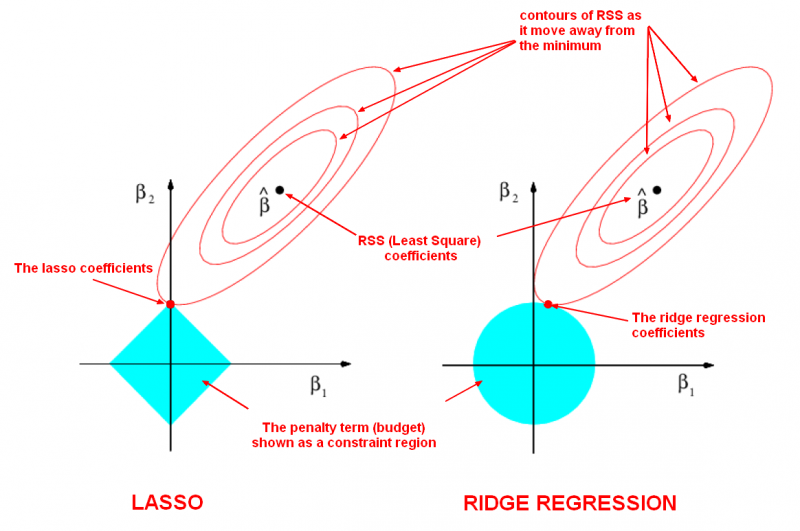
\includegraphics[scale=0.3]{res/lasso_vs_ridge_regression.png}
\caption{Why lasso regression tends to lead to feature sparsity}
\label{lasso-vs-ridge-sparsity}
\end{figure}

Lasso regression ($\mathit{l}_1$-norm) is not differentiable, thus we cannot apply gradient descent as-is.
We split each coefficient into positive and negative parts: rewrite the vector $w = w^{+} - w^{-}$ ($|w| = w^{+} + w^{-}$), and we have this equivalent problem\footnote{whose equivalence can be proved. And this can be plugged in to a quadratic solver to give us $w^{+}$ and $w^{-}$}:

$$
\argmin_{w^{+}, w^{-}}{\frac{1}{n} \sum_{i = 1}^{n}{((w^{+} - w^{-})^{T} x_i - y_i)^2} + \lambda (w^{+} + w^{-})}
$$
subject to $w_i^{+} \geq 0 ~ \forall i$, $w_i^{-} \leq 0 ~ \forall i$

Now we have a constraint and two vectors, to find the minimum, we can use \textbf{projected SGD}\footnote{Normal gradient descent but project / reset each coordinate to the constrained space after each step} or \textbf{coordinate descent}.

Coordinate gradient descent on a vector $w$ works by adjusting only a single $w_i$ in each step, as opposed to possibly alter the entire $w$ in one step as in regular gradient descent.
We iteratively adjust each coordinate several times, where we can pick a random one to adjust, or do cyclic adjustment.

Coordinate gradient descent has a \textbf{closed form solution} for lasso (in the form below\footnote{This form is not differentiable, but it can be shown that for coordinate gradient descent to work there is a weaker condition, which lasso satisfies. \textit{This would indicate that the split into positive and negative shown above is not required, for solving using coordinate gradient descent?}}), where we can use a formula to solve each $w_i$, instead of having to loop over them.

$$
\hat{w}_j = \argmin_{w_j \in \mathbf{R}}{\frac{1}{n} \sum_{i = 1}^{n}{(w^{T} x_i - y_i)^2} + \lambda \norm{w}_1}
$$

\subsection{Elastic nets}

Consider what happens in lasso and ridge regressions when features are linear:
lasso would assign all the weight to the feature with larger scale, and ridge would assign the weights proportional to the features' scales.

It's similar when features are highly correlated (near-linear relationship between features):
think Figure \ref{lasso-vs-ridge-sparsity} instead of parallel lines, we get elongated ellipses, whose intersection with the hypothesis space would reflect the scales of correlated features.

\textbf{Elastic net} combines lasso and ridge penalties.

$$
\hat{w} = \argmin_{w \in \mathbf{R}^{d}}{\frac{1}{n} \sum_{i = 1}^{n}{(w^{T} x_i - y_i)^2} + \lambda_1 \norm{w}_1 + \lambda_2 \norm{w}_2^2}
$$

Geometrically, we end with a hypothesis space like a diamond with edges bulging out (between a circle and a diamond).

\subsection{Regression loss functions}

A \textbf{distance-based loss function} is a loss function ($\mathit{l}(\hat{y}, y) \in \mathbf{R}$) that only depends on the \textbf{residual} $r = \hat{y} - y$.
Most regression losses are distance-based.

Distance-based losses are translation-invariant: $\mathit{l}(\hat{y} + a, y + a) = \mathit{l}(\hat{y}, y)$.

Square loss ($\mathit{l}(r) = r^2$) penalizes outlier points more heavily than absolute (Laplacian) loss ($\mathit{l} = |r|$) does, and is considered less robust.

Downside with absolute loss is that it's not differentiable.

We are able to construct \textbf{Huber loss function} that is robust and differentiable: quadratic for $|r| \leq \delta$ and linear for $|r| > \delta$.

\subsection{Classification loss functions}

If we have action space $\mathbf{A}$ and outcome space $\mathbf{Y}$ both being $\{-1, 1\}$.

\textbf{0-1 loss} for $f: \mathbf{X} \to \{-1, 1\}$:

$$
\mathit{l}(f(x), y) = 1 ~ (f(x) \neq y)
$$

Where $1 ~ (f(x) \neq y)$ denotes score 1 whenever $(f(x) \neq y)$.
\\
\\
If we allow \textbf{real-valued prediction function} $f : \mathbf{X} \to \mathbf{R}$, meaning action space $\mathbf{A} = \mathbf{R}$ where the value represents confidence of our prediction.

We can define \textbf{margin} $m$ as $m = y \hat{y}$, where $\hat{y}$ stands for the predicted score.
We want to maximize the margin.
Most classification losses are \textbf{margin-based}.

Empirical risk for 0-1 loss is

$$
\hat{R}_n(f) = \frac{1}{n} \sum_{i = 1}^{n}{1}~(y_i f(x_i) \leq 0)
$$

$\hat{R}_n(f)$ is non-convex, not differentiable, discontinuous, and its optimization is NP-hard.
\\
\\
\textbf{SVM/Hinge loss} is defined as

$$
\mathit{l}_{Hinge} = max\{ 1 - m, 0 \} = (1 - m)_+
$$

It is a convex, upper bound on 0-1 loss, and not differentiable at $m = 1$.
And we have \textbf{margin error} when $m < 1$.

Using hinge loss function, we define \textbf{soft margin linear support vector machine} (a constrained empirical risk minimizer) as

$$
\argmin_{w \in \mathbf{R}^{d}}{\frac{1}{n} \sum_{i = 1}^{n}{(1 - y_i f_w (x_i))_+} + \lambda \norm{w}_2^2}
$$

With $l2$ regularization, and hypothesis space is linear $\{f(x) = w^{T} x | w \in \mathbf{R}^d\}$.
\\
\\
\textbf{Logistic/log loss} is defined as 

$$
\mathit{l}_{Logistic} = \text{log}(1 + e^{-m})
$$

It always wants more margin, and is differentiable.
\\
\\
0-1 loss, hinge and Logistic loss functions are illustrated in Figure \ref{logistic-hinge-01-loss} \footnote{http://fa.bianp.net/blog/2013/loss-functions-for-ordinal-regression/}.

\begin{figure}[h]
\centering
\includegraphics[scale=0.3]{res/logistic-hinge-01-loss.png}
\caption{0-1 loss, hinge loss and Logistic loss functions}
\label{logistic-hinge-01-loss}
\end{figure}

\subsection{SVM and Lagrangian duality}

Adding a \textbf{bias} term $b$ to the constrained empirical risk minimizer of \textbf{support vector machine}, we have

$$
\argmin_{w \in \mathbf{R}^{d}, ~ b \in \mathbf{R}}{\frac{c}{n} \sum_{i = 1}^{n}{\text{max}(0, 1 - y_i (w^{T} x_i + b))} + \frac{1}{2} {\norm{w}_2^2}}
$$

whose solution gives us the SVM prediction function.
$c$ is a constant that can be tweaked to decide how much regularization matters.

This problem is not differentiable due to $max$.
We can turn it into an equivalent problem.

\begin{align*}
\text{minimize}   ~~& \frac{c}{n} \sum_{i = 1}^{n}{\xi_i} + \frac{1}{2} {\norm{w}_2^2} \\
\text{subject to} ~~& -\xi_i &\leq 0, ~ \forall i \in \{1, \dots n\} \\
                  & (1 - y_i (w^{T} x_i + b)) - \xi_i &\leq 0, ~ \forall i \in \{1, \dots n\}
\end{align*}

This has a differentiable objective function, $n + d + 1$ unknowns and $2 d$ affine constraints.
This can be solved by off-the-shelf QP solver.
$\sum_{i = 1}^{n}{\xi_i}$ now represents the margin loss.

We apply \textbf{Lagrangian multiplier} to the constrained optimization problem to get the following

\begin{align*}
L(w, b, \xi, \alpha, \lambda) &= \frac{1}{2} {\norm{w}_2^2} + \frac{c}{n} \sum_{i = 1}^{n}{\xi_i} + \sum_{i = 1}^{n}{\alpha_i (1 - y_i (w^{T} x_i + b) - \xi_i)} - \sum_{i = 1}^{n}{\lambda_i \xi_i} \\
                              &= \frac{1}{2} w^{T} w + \sum_{i = 1}^{n}{\xi_i (\frac{c}{n} - \alpha_i - \lambda_i)} + \sum_{i = 1}^{n}{\alpha_i (1 - y_i (w^{T} x_i + b))}
\end{align*}

Its \textbf{primal} and \textbf{dual problems} look like

\begin{align*}
p^* &= \minf_{w, \xi. b} \msup_{\alpha, \lambda \geq 0} L(w, b, \xi, \alpha, \lambda) \\
    &\geq \msup_{\alpha, \lambda \geq 0} \minf_{w, \xi. b} L(w, b, \xi, \alpha, \lambda) \\
    &= d^*
\end{align*}

This satisfies strong duality by \textbf{Slater's constraint qualification}.
\footnote{Where a convex problem + affine constraints $\implies$ strong duality iff problem is \textbf{feasible}.
This problem is feasible if we simply let $w = b = 0$ and $\xi_i = 1 ~ \forall i \in \{1, \dots n\}$}

The \textbf{Lagrangian dual function} then becomes

\begin{align*}
g(\alpha, \lambda) &= \minf_{w, \xi. b} L(w, b, \xi, \alpha, \lambda) \\
                   &= \minf_{w, \xi. b} (\frac{1}{2} w^{T} w + \sum_{i = 1}^{n}{\xi_i (\frac{c}{n} - \alpha_i - \lambda_i)} + \sum_{i = 1}^{n}{\alpha_i (1 - y_i (w^{T} x_i + b))})
\end{align*}

This is convex and differentiable: quadratic in $w$, and linear in $\xi_i$ and $b$.
The global minima is at $\frac{\partial L}{\partial w} = 0$, $\frac{\partial L}{\partial \xi} = 0$, $\frac{\partial L}{\partial b} = 0$.

Solving the three partial derivations (\textbf{first order conditions}), we have

\begin{align*}
\frac{\partial L}{\partial w} = 0   \implies & ~w = \sum_{i = 1}^{n}{\alpha_i y_i x_i} \\
\frac{\partial L}{\partial \xi} = 0 \implies & ~\alpha_i + \lambda_i = \frac{c}{n} \\
\frac{\partial L}{\partial b} = 0   \implies & ~\sum_{i = 1}^{n}{\alpha_i y_i = 0}
\end{align*}

Replacing the $w$, $\xi$ and $b$s from the \textbf{dual function}, the \textbf{dual problem} then becomes

\begin{align*}
\msup_{\alpha} ~ ~ & \sum_{i = 1}^{n}{\alpha_i} - \frac{1}{2} \sum_{i = 1}^{n}{\alpha_i \alpha_j y_i y_j x_j^{T} x_i} \\
s.t.               & \sum_{i = 1}^{n}{\alpha_i y_i} = 0 \\
                   & \alpha_i \in \begin{bmatrix}0, \frac{c}{n}\end{bmatrix} ~ ~ \forall i \in \{1, \dots n\}
\end{align*}

Note
\begin{itemize}
  \item Given a solution $\alpha^*$ to dual, primal solution is $w^* = \sum_{i = 1}^{n}{\alpha_i^* y_i x_i}$.
  \item $w^*$ is a linear combination of the data $x_1, \dots x_n$. The $x_i$'s corresponding to $\alpha_i^* > 0$ are called \textbf{support vectors}.
  \item $\alpha^* \in \begin{bmatrix}0, \frac{c}{n}\end{bmatrix}$, so $c$ controls the maximum weight on each sample. This is \textbf{robust}.
  \item This is a quadratic objective with $n$ unknowns and $n + 1$ constraints.
  \item Efficient minimization algorithm, sequential minimal optimization, exists.
\end{itemize}

Since we have \textbf{strong duality}, \textbf{complementary slackness} holds, where the Lagrangian multiplier $\times$ the constraint function is 0.

\begin{align*}
\alpha_i^* (1 - y_i f^*(x_i) - \xi_i)                    &= 0 \\
\lambda_i^* \xi^*_i = (\frac{c}{n} - \alpha_i^*) \xi_i^* &= 0
\end{align*}

This means

\begin{itemize}
  \item $y_i f^*(x_i) > 1 \implies \alpha_i^* = 0, ~\xi_i^* = 0$
  \item $y_i f^*(x_i) < 1 \implies \alpha_i^* = \frac{c}{n}, ~\xi_i^* > 0$
  \item $y_i f^*(x_i) = 1 \implies \alpha_i^* \in \begin{bmatrix}0, ~\frac{c}{n}\end{bmatrix}$
  \item $\alpha_i^* = 0   \implies \xi_i^* = 0$ (margin loss is 0), so $y_i f^*(x_i) \geq 1$
  \item $\alpha_i^* = \frac{c}{n} \implies y_i f^*(x_i) \leq 1$
  \item $\alpha_i^* \in \begin{pmatrix}0, \frac{c}{n}\end{pmatrix} \implies y_i f^*(x_i) = 1$
\end{itemize}

Suppose we have an $i$ s.t. $\alpha_i^* \in \begin{pmatrix}0, \frac{c}{n}\end{pmatrix}$, using the complementary slackness conditions we can solve the bias term $b^*$, whose value stays the same for any choice of $i$ satisfying $\alpha_i^* \in \begin{pmatrix}0, \frac{c}{n}\end{pmatrix}$.
\footnote{With numerical error, it's more rubust to average over all eligible $i$ and use the mean of resulting $b^*$}

$$
b^* = y_i - x_i^{T} w^*
$$

If there are no such $\alpha_i^*$s, then we have a degenerate SVM training problem.

\subsection{Level sets / contours, sublevel sets and convex optimization}

Let $f : \mathbf{R}^d \to \mathbf{R}$ be a function.
A \textbf{level set} or \textbf{contour line} for the value $c$ is the set of points $x \in \mathbf{R}^d$ for which $f(x) = c$.

A \textbf{sublevel set} for the value $c$ is the set of points $x \in \mathbf{R}^d$ for which $f(x) \leq c$.

If $f : \mathbf{R}^d \to \mathbf{R}$ is \textbf{convex}, then sublevel sets are convex.
Level sets and superlevel sets of convex functions are not generally convex, hence, the \textbf{standard form of convex optimization problem} uses $\leq 0$ to express constraints.

The \textbf{implicit form of convex optimization problem} goes as

\begin{align*}
\text{minimize}   & ~ ~ f(x) \\
\text{subject to} & ~ ~ x \in C
\end{align*}

where $f$ is a convex function and $C$ is a convex set.

Also, intersection of convex sets is convex.

\subsection{First-order approximation}

Suppose $f : \mathbf{R}^d \to \mathbf{R}$ is differentiable.

We can use \textbf{linear} / \textbf{first-order approximation} to predict $f(y)$ given $f(x)$ and $\bigtriangledown f(x)$

$$
f(y) \approx f(x) + \bigtriangledown f(x)^{T} (y - x)
$$
\\
\\
Now suppose $f : \mathbf{R}^d \to \mathbf{R}$ is convex and differentiable.

The linear approximation to $f$ at $x$ is a \textbf{global underestimator} of $f$.

$$
\forall ~ x, y \in \mathbf{R}^d, ~ ~ f(y) \geq f(x) + \bigtriangledown f(x)^{T} (y - x)
$$

And if $\bigtriangledown f(x) = 0$ then $x$ is a global minimizer of $f$ \footnote{Where local information gives global information!}.

\subsection{Subgradients}

A vector $g \in \mathbf{R}^d$ is a \textbf{subgradient} of $f : \mathbf{R}^d \to \mathbf{R}$ at $x$ if $\forall ~ z$,

$$
f(z) \geq f(x) + g^{T} (z - x)
$$

$f$ is \textbf{subdifferentiable} at $x$ if $\exists$ at least one subgradient at $x$.

The set of all subgradients at $x$ is called the \textbf{subdifferential}: $\partial f(x)$

$f$ is convex and differentiable $\implies \partial f(x) = \{ \bigtriangledown f(x) \}$.
At any point $x$, there can be $0$, $1$, or infinite many subgradients.
$\partial f(x) = \emptyset \implies f$ is not convex.

If $0 \in \partial f(x)$, then $x$ is a \textbf{global minimizer} of $f$.

As a reminder, for function $f : \mathbf{R}^d \to R$,
\begin{itemize}
  \item graph of function lives in $\mathbf{R}^{d + 1}$
  \item gradient, subgradient of $f$ live in $\mathbf{R}^d$, and
  \item contours, level sets, sublevel sets are in $\mathbf{R}^d$
\end{itemize}

Gradient at $x$ is orthogonal to level set at $x$. (assuming $f$ continuously differentiable.)
\\
\\
Now to figure out the \textbf{direction} on which to do a subgradient descent.

Let $f : \mathbf{R}^d \to \mathbf{R}$ have a subgradient $g$ at $x_0$, hyperplane $H$ orthogonal to $g$ at $x_0$ must \textbf{support} the level set $S = \{ x \in \mathbf{R}^d | f(x) = f(x_0) \}$, meaning $H$ contains $x_0$ and all of $S$ lies on one side of $H$.
The proof of which\footnote{Using the definition of subgradient, and inner product $g^T \cdot (y - x_0) > 0$ if $y$ is on the side $g$ points in} suggests the following:

Points on subgradient $g$ side of $H$ have larger $f$-values than $f(x_0)$, and points on $-g$ side may not have smaller $f$-values, meaning $-g$ may not be a descent direction.
\\
\\
In \textbf{subgradient descent}, suppose we repeatedly step in a negative subgradient direction $x = x_0 - t g$ where $t > 0$ is the step size and $g \in \partial f(x_0)$.

We can prove $-g$ gets us closer to minimizer.
Meaning, suppose $f$ is convex, let $x = x_0 - t g$ for $g \in \partial f(x_0)$, and let $z$ be any point for which $f(z) < f(x_0)$, then for small enough $t > 0$, $\norm{x - z}_2 < \norm{x_0 - z}_2$.

\textbf{Proof:}
\begin{align*}
\norm{x - z}_2^2 &= \norm{x_0 - tg - z}_2^2 \\
                 &= \norm{x_0 - z}_2^2 - 2 t g^T (x_0 - z) + t^2 \norm{g}_2^2 \\
                 &\leq \norm{x_0 - z}_2^2 - 2 t (f(x_0) - f(z)) + t^2 \norm{g}_2^2
\end{align*}

Consider

$$
g(t) = - 2 t (f(x_0) - f(z)) + t^2 \norm{g}_2^2
$$

It's a convex quadratic facing upwards, has zeros at $t = 0$ and $t = 2 (f(x_0) - f(z)) / \norm{g}_2^2 > 0$, so

$$
g(t) < 0 ~\forall ~ t \in \begin{pmatrix} 0, \frac{2 (f(x_0) - f(x))}{\norm{g}_2^2} \end{pmatrix}
$$

Thus we have $-g$ gets us closer to a smaller $f(z)$.

\subsection{Features extraction}

Mapping an input space $\mathbf{X}$ (sound wave, image, DNA sequence) to a vector $\mathbf{R}^d$ is called \textbf{feature extraction} or \textbf{featurization}.

A \textbf{feature template} is a group of features all computed in a similar way (e.g. $last\_three\_chars\_of(x) = \_\_\_$).\footnote{With regularization, our resulting prediction function won't be too complicated.}

A \textbf{one-hot encoding} is a feature template that always has exactly one non-zero value.

Features can be encoded with an array (good for dense features), or a map (good for sparse features).

Some factors to consider when featurizing
\begin{itemize}
  \item Non-monotonicity. E.g. temperature as a feature for health prediction, health is not monotonic with temperature. We can transform the input $\Phi{x} = [1, \{temperature(x) - 37\}^2]$\footnote{Array representation of features, where $1$ is a bias term}, but this would require domain knowledge, instead, we could do $\Phi(x) = [1, temperature(x), \{temperature(x)\}^2]$, where having one extra feature, we increase the flexibility and make it easier to use.\footnote{Think less, make the computer do more}
  \item Saturation. E.g. find products relevant to user's query, where given a product $x$, we have a feature map $\Phi(x) = [1, N(x)]$ where $N(x) = \text{number of people who bought x}$. However at some point $x$ should saturate: a product bought 50000 times is not necessarily 10 times more relevant than a product bought 5000 times, as a linear model would suggest. We could do $log(1 + N(x))$, or $arctan(x)$\footnote{A sigmoid function. Note how this transformation does not need to be convex.} to slow down the growth. Or we could do a discretization, like $\Phi(x) = [1 (x < 10), 1 (10 \leq x < 100), 1 (100 \leq x)]$\footnote{Where if not bucketed carefully, buckets with few items will have coefficients $0$, due to regularization. Instead, we could have $\Phi(x) = [1 (x \geq 5), 1 (x \geq 10), 1 (x \geq 100)], where a small bucket would fall back to the previous feature.$}.
  \item Interaction. E.g. predicting health with weight and height, it's not that they individually matter, but rather weight relative to height. You can add a cross term $h(x)w(x)$, making $\Phi(x) = [1, h(x), w(x), h^2(x), x^2(x), h(x)w(x)]$
\end{itemize}

A \textbf{predicate} of the input space is a function $P : \mathbf{X} \to \{\text{True},~\text{False}\}$.

What about given features $\Phi(x) = [x_1, x_2]$, we want to classify if a point will fall into a circle in the two-dimensional input space? We could add $x_1^2 + x_2^2$ as another feature.

Similaryly, output space can be transformed as well.

We essentially grow the (linear) hypothesis space by adding more features.

\subsection{Kernel methods}

From a high level, goal is to allow access to huge feature spaces without suffering heavy computational cost.

With featurization, we can map input space $\mathbf{X} \subset \mathbf{R}^n$ to $\mathbf{R}^d$\footnote{And as it would seem, this optimization makes sense when $n < d$}, and the hypothesis space is of affine functions on feature space looks like

$$
\mathbf{H} = \{ x \to w^{T}\Phi{x} + b | w \in \mathbf{R}^d, b \in \mathbf{R} \}
$$

To get expressive hypothesis spaces using linear models, we need high-dimensional feature spaces (say, adding in all $x_i^{k_i}$ where $\sum{k_i} \leq C$).
This complicates computation, and may cause overfitting.
Overfitting can be handled with regularization, and kernel methods can help with memory and computational costs.

For example, recall a featurized SVM prediction function, which is the solution to the following

$$
\argmin_{w \in \mathbf{R}^d, b \in \mathbf{R}} (\frac{1}{2} w^{T} w + \frac{c}{n} \sum_{i = 1}^{n}{(1 - y_i [w^T \Phi(x_i) + b])_+}
$$

whose dual is

\begin{align*}
\msup_{\alpha} ~ ~ & \sum_{i = 1}^{n}{\alpha_i} - \frac{1}{2} \sum_{i,j = 1}^{n}{\alpha_i \alpha_j y_i y_j \Phi(x_j)^{T} \Phi(x_i)} \\
s.t.               & \sum_{i = 1}^{n}{\alpha_i y_i} = 0 \\
                   & \alpha_i \in \begin{bmatrix}0, \frac{c}{n}\end{bmatrix} ~ ~ \forall i \in \{1, \dots n\}
\end{align*}

Where $\Phi{x}$ only shows up as inner products with other $x$s.

A method is \textbf{kernerlized} if inputs only appear inside inner products. $\langle \Phi(x) , \Phi(x') \rangle$ for $x, x' \in \mathbf{X}$.
The \textbf{kernel function} corresponding to $\Phi$ and inner product $\langle . , . \rangle$ is

$$
k(x, x') = \langle \Phi(x) , \Phi(x') \rangle
$$

For example, consider quadratic feature map for $x = (x_1, \dots x_d) \in \mathbf{R}^d$

$$
\Phi(x) = (x_1, \dots x_d, x_1^2, \dots x_d^2, \sqrt{2} x_1 x_2, \dots, \sqrt{2} x_{d - 1} x_d)^T
$$

has dimension $O(d^2)$, but for any $x, x' \in \mathbf{R}^d$

$$
k(x, x') = \langle \Phi(x), \Phi(x') \rangle = \langle x, x' \rangle + \langle x, x' \rangle^2
$$

Bringing down the computation cost from $O(d^2)$ to $O(d)$.\footnote{Often useful to think of the kernel function as a \textbf{similarity score}}

Continuing on with the SVM example, with linear kernel $k(x, x') = x^T x'$, we define the \textbf{kernel matrix} (\textbf{Gram matrix}) as such:

$$
K = (\langle x_i, x_j \rangle)_{i, j} =
\begin{pmatrix}
\langle x_1, x_1 \rangle \dots \langle x_1, x_n \rangle \\
\dots \\
\langle x_n, x_1 \rangle \dots \langle x_n, x_n \rangle \\
\end{pmatrix}
$$

Then for the standard Euclidean inner product $\langle x_i, x_j \rangle = x_i^T x_j$, we have

$$
K = X X^T
$$

Where $X = (x_1, \dots x_n)^T$, an $n \times d$ vector, and $K$ is all the $Phi(x)-$terms we are interested in.\footnote{Recall with ridge regression, we worked with $X^T X$, which is $d \times d$, meaning we are interested in kernel methods when $n \leq d$}

And the dual problem becomes

\begin{align*}
\msup_{\alpha} ~ ~ & \sum_{i = 1}^{n}{\alpha_i} - \frac{1}{2} \sum_{i,j = 1}^{n}{\alpha_i \alpha_j y_i y_j K_{ji}} \\
s.t.               & \sum_{i = 1}^{n}{\alpha_i y_i} = 0 \\
                   & \alpha_i \in \begin{bmatrix}0, \frac{c}{n}\end{bmatrix} ~ ~ \forall i \in \{1, \dots n\}
\end{align*}

This also gives us the flexibility to change kernels to a different $K$ of $n \times n$ dimension, which can, e.g., correspond to a high dimensional feature space.
This is \textbf{kernel trick}.
\\
\\
And there are other non-linear kernels, our quadratic example earlier and \textbf{polynomial kernel} $k(x, x') = (1 + \langle x, x' \rangle)^M$, which corresponds to a feature map with all monomials up to degree $M$, the computational cost of the kernel does not grow with $M$, while plugging in the featurized terms directly the computational cost grows rapidly with $M$.

And \textbf{Radial Basis Function / Gaussian kernel}, $\forall x, x' \in \mathbf{R}^d$

$$
k(w, x) = e^{- \frac{\norm{x - x'}^2}{2 \sigma^2}}
$$\footnote{Note how this acts like a similarity score, and with this kernel, your featurization dimension $d$ may grow, but to compute the kernel is always $n \times n$ where $n$ is the number of data points.}


\subsection{Representer theorem and its usage in kernelization}

Consider SVM objective function in a more general term,

$$
\argmin_{w \in \mathbf{H}}{J(w)}
$$

And let $J(w)$ be

$$
J(w) = R(\norm{w}) + L(\langle w , \Phi(x_1) \rangle , \dots , \langle w , \Phi(x_n) \rangle)
$$

Where $\norm{.}$ corresponds to the inner product on space $\mathbf{H}$.
$R : [0, \infty) \to \mathbf{R}$ is the regularization term and $L : \mathbf{R}^n \to \mathbf{R}$ is the loss term.\footnote{Each inner product represents a (linear) prediction. Ridge regression and SVM are both of this form. Lasso is not, as $l_1$ norm does not correspond to an inner product.}

If $J(w)$ has a minimizer, then it has a minimizer of the form $w^* = \sum_{i = 1}^{n}{\alpha_i \Phi(x_i)}$.\footnote{This is the same conclusion we reached at the end of SVM: $w^*$ is a linear combination of features. This can be proved using Pythagorean theorem and projection theorem: do a projection from $w^*$ to $M$, span of the data}

With this, we don't have to search over the feature space $w^*$ is in, $\mathbf{R}^d$, but rather having computed the $n$ $\Phi(x_i)$s, we search over that space of $n$ dimensions.
This lets you deal with infinite dimensional feature space.

As an example, a kernelized objective function for SVM looks like

$$
\argmin_{\alpha \in \mathbf{R}^n} R(\sqrt{\alpha^T K \alpha}) + L(K \alpha)
$$

Where there is no direct access to $\Phi(x_i)$, and all references are via kernel matrix $K$.


\subsection{Performance evaluation}

Intuition,
\begin{itemize}
\item Always spend some time building a linear baseline model. (lasso / ridge / elastic net regression; l1 / l2 regularized logistic regression or svm)
\item Prefer simpler models if performance is the same.
\item Consider building an oracle model, which is helpful to get an upper bound on achievable performance. E.g. fit your validation data without regularization. This can give estimate of the approximation error of our hypothesis space.
\end{itemize}

\textbf{Confusion matrix} for binary classification problem, the 4-cell matrix of true / false positive / negatives.

\begin{itemize}
\item \textbf{True positive}: predicted positive, and it's right
\item \textbf{True negative}: predicted negative, and it's right
\item \textbf{False positive / type 1 error}: predicted positive, and it's wrong
\item \textbf{False negative / type 2 error}: predicted negative, and it's wrong
\end{itemize}

Criteria based on the confusion matrix,
\begin{itemize}
\item \textbf{Accuracy} $(TP + TN) / (TP + TN + FP + FN)$
\item \textbf{Error rate} $(FP + FN) / (TP + TN + FP + FN)$
\item $\text{Accuracy} + \text{Error rate} = 1$.
\item Accuracy by itself is often not enough, consider a no-information classifier (always produced 0, e.g.) on a distribution that's predominantly one-sided (e.g. 0).
\item \textbf{Precision} $TP / (TP + FP)$: high precision means low false alarm rate.
\item \textbf{True positive rate / recall / sensitivity} $TP / (TP + FN)$: high recall means you are not missing many positives.
\item \textbf{False negative rate / miss rate} $FN / (FN + TP)$
\item \textbf{False positive rate / fall-out / false-alarm rate} $FP / (FP + TN)$
\item \textbf{True negative rate / specificity} $TN / (FP + TN)$
\item \textbf{$F_1$ score}. $F_1 = 2 \frac{precision \cdot recall}{precision + recall}$. $F_{\beta}$. Weigh towards precision or recall
\end{itemize}

In a classification problem, the real-valued prediction function (score function) does not have to be thresholded at 0\footnote{$> 0$ predict positive, $< 0$ predict negative}.
Thresholding the score function differently causes the performance metrics to shift.
We can threshold it at a value to meet our performance goals, e.g. $recall > 80\%$.

Measurement curves based on these rates.
\begin{itemize}
\item \textbf{Precision-recall curve}: as you change the threshold, how precision and recall change.
\item \textbf{Receiver-operation characteristic (ROC) curve}: as you change threshold, how TP rate and FP rate change.
\item \textbf{AUC / AUC ROC}: area under the ROC curve.
\end{itemize}

\subsection{Probablistic modeling}

Instead of producing a single value or classification (regression or classification), produce a probability distribution of values, with which we can decide how likely a test data point is.
This is applicable in e.g. anonamaly detection.

The approach usually entails selecting a particular probability distribution, and fit the samples to derive the parameters of that distribution. (E.g. the mean value of Poisson distribution)

\textbf{Stratification} means partitioning our input data into groups, and treat each group separately.
E.g. we stratify each symbol traded into time ranges like 9:30A to 10:30A on every weekday, and train a model for that particular time range.

\textbf{Bucketing / binning} is the opposite of stratification, where we combine natural groups of data into a single group, and train a model for that single group.
E.g. we can bucket multiple tech stock symbols into one group, and train one model to predict their overall price movement.

Stratification brings out specificity (also more bias), bucketing smoothes bias out but lose specificity.


\subsection{Neural nets}

Linear prediction functions, like SVM, ridge, lasso generate feature vector $\Phi(x)$ by hand, and learn parameter vector $w$ from data.
A neural net adds \textbf{hidden nodes} between the $\Phi(x)$ and score.
Multi-layer perceptron, e.g. in this two-layer representation (two affine combinations):

\begin{align*}
h_i   &= \sigma(v_i^T \Phi(x)) \\
score &= w^T h + b
\end{align*}

where $\sigma$ is a nonlinear \textbf{activation function}, and we need to learn the vectors $v_i$ (with a bias term), $w$, and scalar $b$.
We can add hidden nodes, hidden layers, etc, where $>1$ hidden layer is a deep network.

\textbf{Hyperbolic tangent} is a common activation function.

$$
\sigma(x) = tanh(x)
$$

\textbf{Rectified linear function} (ReLU) is another. ReLU in practice often works better.

$$
\sigma(x) = max(0, x)
$$

One way to think about neural nets is that it's learning the non-linear featurization functions we want to create.
(From the hidden layer $h_i$ to $score$ looks just like learning in a linear context, and neural nets learn $\Phi(x)$ to $h_i$ as well).

Our objective function (with $tanh$) is then differentiable w.r.t. all parameters (we can use gradient descent), but not convex.
In practice gradient descent seems sufficient.

\textbf{Universal approximation theorem}: a neural network with one (possibly huge) hidden layer can uniformly approximate any continuous function on a compact set iff the activation function is not a polynomial. (the bias term is necessary)

\subsection{Multinomial logistic regression}




\section{Exercises}

\subsection{Deriving gradient affine form}

1. Given $f(w) = c^{t} w$ , $\bigtriangledown f(w)$?

$$
f'(x; u) = \lim\limits_{h \to 0}{\frac{f(w + hu) - f(w)}{h}} = \lim\limits_{h \to 0}{\frac{c^{T} h u}{h}} = c^{T} u
$$

This shows

$$
\bigtriangledown f(x) = c
$$

2. Given $f(w) = w^{T} A w$ , $\bigtriangledown f(w)$?

\begin{align*}
f'(w; u) &= \lim\limits_{h \to 0}{\frac{f(w + hu) - f(w)}{h}} \\
         &= \lim\limits_{h \to 0}{\frac{(w + hu)^{T} A (w + hu) - w^{T} A w}{h}} \\
         &= \lim\limits_{h \to 0}{ \frac{w^{T} A w + h w^{T} u + h u^{T} A w + h^2 u^{T} A u - w^{T} A w}{h} } \\
         &= u^{T} A w + w^{T} A u \\
         &= w^{T} A^{T} u + w^{T} A u
\end{align*}

This shows
$$
\bigtriangledown f(x) = (w^{T} A^{T} + w^{T} A)^{T} = (A + A^{T}) w
$$

3. Given $f(w) = \norm{Aw - y}_2^2$ , $\bigtriangledown f(w)$?

$$
f(w) = \norm{Aw - y}_2^2 = (Aw - y)^{T} (Aw - y)
$$

\begin{align*}
f'(w; u) &= \lim\limits_{h \to 0}{\frac{(A (w + hu) - y)^{T} (A (w + hu) - y) - (Aw - y)^{T} (Aw - y)}{h}} \\
         &= \lim\limits_{h \to 0}{ (A (w + hu) - y)^{T} A u + (A u)^{T} (A (w + hu) - y)} \\
         &= (A w - y)^{T} A u + (A u)^{T} (A w - y) \\
         &= 2 (A w - y)^{T} A u
\end{align*}

This shows

$$
\bigtriangledown f(x) = 2 ((A w - y)^{T} A)^{T} = 2 A^{T} (A w - y) = 2 A^{T} A w - 2 A^{T} y
$$

4. Given $f(w) = \norm{Aw - y}_2^2 + \lambda \norm{w}_2^2$ , express $f(w) = \norm{Bw - z}_2^2$?

The gradient of the two need to be the same, using previous result, we need to solve

$$
\begin{cases}
A^{T} A + \lambda &= B^{T} B \\
          A^{T} y &= B^{T} z
\end{cases}
$$

Note the equivalence between extending a matrix and addition, let

$$
B = \begin{pmatrix} A \\ \sqrt{\lambda} I_{n \times n} \end{pmatrix} ~ \text{and} ~ z = \begin{pmatrix} y \\ 0_{n \times 1} \end{pmatrix}
$$

written in block-matrix form.

\subsection{Recap: linear regression with square loss}


\end{document}
